%\documentclass{beamer}
\documentclass[11pt]{beamer}

%\usepackage[english]{babel}
% or whatever
% ESPAÑOL 

\usepackage[spanish]{babel}
\usepackage{tikz}

\usepackage[utf8]{inputenc}
%\usepackage[latin1]{inputenc}
% or whatever

%\usepackage{times}


%\usepackage[T1]{fontenc}
% Or whatever. Note that the encoding and the font should match. If T1
% does not look nice, try deleting the line with the fontenc.

%\usepackage{pgf,pgfarrows,pgfnodes,pgfautomata,pgfheaps}
%\usepackage{pgf,pgfarrows}
\usepackage{pgfarrows}
\usepackage{color}
\usepackage{epsfig}
\usepackage{algoritmo}
\usepackage{hyperref}
%%\usepackage{graphicx}

\usepackage{amssymb, amsmath, amsbsy} % librerias ams

\usepackage{dirtree}


%% Numbered captions
\setbeamertemplate{caption}[numbered]

\mode<presentation>
{
% \usetheme{Warsaw}
  % or ...
%  \usetheme{Rochester}
%%  \usetheme{Pittsburgh}
%  \usetheme{Montpellier}
%  \usetheme{Malmoe}
%  \usetheme{Madrid}
%  \usetheme{Luebeck}
%%  \usetheme{JuanLesPins}
%  \usetheme{default}
%  \usetheme{Copenhagen}
%  \usetheme{CambridgeUS}
%  \usetheme{boxes}
%  \usetheme{Boadilla}
%%  \usetheme{Bergen}
%  \usetheme{Antibes}
%  \usetheme{AnnArbor}
  
\setbeamercovered{transparent}
 % or whatever (possibly just delete it)
 
%\usecolortheme{albatross}
%\usecolortheme{beaver}
%\usecolortheme{crane}
%\usecolortheme{dolphin}
%%\usecolortheme{dove}
%\usecolortheme{default}
%%%\usecolortheme{seagull}
%\usecolortheme{seahorse}
%\usecolortheme{whale}

\useinnertheme[shadow=true]{rounded}
\usecolortheme{orchid}
\usecolortheme{whale}
%%\usecolortheme{wolverine}

\definecolor{steelblue}{rgb}{0.27, 0.51, 0.71}
\definecolor{crimson}{rgb}{0.86, 0.08, 0.24}
\definecolor{navyblue}{rgb}{0.0, 0.0, 0.5}
\definecolor{lightgreen}{rgb}{0.56, 0.93, 0.56}
\definecolor{darkkhaki}{rgb}{0.74, 0.72, 0.42}
\definecolor{darkcerulean}{rgb}{0.03, 0.27, 0.49}
\colorlet{verde-oscuro}{green!20!black}
\colorlet{verde}{green!50!black}

\colorlet{marron-oscuro}{brown!20!black}
\colorlet{marron}{brown!50!black}

\colorlet{amarillo-claro}{yellow!50!white}

\colorlet{rosa}{red!50!white}


\setbeamertemplate{headline}
{%
 \begin{beamercolorbox}{section in head/foot}
  \vskip5pt
  \hskip5pt
  \insertshorttitle{\large Programación Declarativa}
   %\hskip20pt
  \hfill 
  \insertshorttitle{\large Representación gráfica en Racket\hskip5pt}
  \vskip5pt
 \end{beamercolorbox}%
}

\setbeamertemplate{footline}
{%
 \begin{beamercolorbox}{section in head/foot}
  \vskip2pt
  \hskip10pt
  \insertshorttitle{Universidad de Córdoba}
  \hskip45pt
  \insertshorttitle{4º Grado Ingeniería Informática: Computación}
  \hskip70pt
  \insertpagenumber 
  \hskip2pt 
  / 
  \hskip2pt 
  \insertpresentationendpage
  \vskip2pt 
 \end{beamercolorbox}%
}

}

\newtheorem{teorema}{Teorema}[theorem]
\newtheorem{demostracion}{Demostración}[theorem]
\newtheorem{ejemplo}{\textcolor{green}{Ejemplo}}[theorem]
\newtheorem{ejemplos}{\textcolor{green}{Ejemplos}}[theorem]
\newtheorem{ejercicio}{\textcolor{brown}{Ejercicio}}[theorem]
\newtheorem{definicion}{\textcolor{yellow}{Definición}}[theorem]
\newtheorem{nota}{\textcolor{amarillo-claro}{Nota}}[theorem]
\newtheorem{notas}{\textcolor{amarillo-claro}{Notas}}[theorem]
\newtheorem{algoritmo}{\textcolor{red}{Algoritmo}}[theorem]


%\title[Short Paper Title] % (optional, use only with long paper titles)
\title[] % (optional, use only with long paper titles)
{Hundir la flota}

\subtitle
{Representación gráfica en Racket}
%%\small{\emph{Asignatura de Programación Declarativa}}}
\author{Carlos Lucena Robles}% (optional, use only with lots of authors)

%{F.~Author\inst{1} \and S.~Another\inst{2}}
% - Use the \inst{?} command only if the authors have different
%   affiliation.

\institute[Universities of Somewhere and Elsewhere] % (optional, but mostly needed)
{
  % \inst{1}%
  Curso 4º de Grado de Ingeniería Informática\\
  Programación Declarativa. 1º Cuatrimestre\\
  Escuela Politécnica Superior\\
  Universidad de Córdoba
  % \and
  % \inst{2}%
  % Department of Theoretical Philosophy\\
  % University of Elsewhere
 }
% - Use the \inst command only if there are several affiliations.
% - Keep it simple, no one is interested in your street address.

%\date[Short Occasion] % (optional)
%{Date / Occasion}
\date{Curso académico 2023 - 2024 \\
Córdoba, 8 de enero de 2024}

%\subject{Talks}
\subject{Hundir la flota. Representación gráfica en Racket}
% This is only inserted into the PDF information catalog. Can be left
% out. 



% If you have a file called "university-logo-filename.xxx", where xxx
% is a graphic format that can be processed by latex or pdflatex,
% resp., then you can add a logo as follows:

% \pgfdeclareimage[height=0.5cm]{University-logo}{university-logo-filename}
%\logo{\pgfuseimage{university-logo}}



% Delete this, if you do not want the table of contents to pop up at
% the beginning of each subsection:


%\AtBeginSection[]
%{
 % \begin{frame}<beamer>
 %   \frametitle{Contenido del Trabajo}
    %\tableofcontents[currentsection,currentsubsection]
 %   \tableofcontents[currentsection,hideallsubsections]
%  \end{frame}
%}

%\AtBeginSubsection[]
%{
 % \begin{frame}<beamer>
%   \frametitle{Contenido del apartado}
   %\tableofcontents[currentsection,currentsubsection,hideothersubsections]
%   \tableofcontents[currentsubsection,subsectionstyle=show/shaded/hide]
   
%  \end{frame}
%}


%\AtBeginSubsubsection[]
%{
%  \begin{frame}<beamer>
%   \frametitle{Contenido de la sección}
%   %\tableofcontents[currentsection,currentsubsection,hideothersubsections]
%   \tableofcontents[currentsubsubsection,subsubsectionstyle=show/shaded/hide]
   
%  \end{frame}
%}


% If you wish to uncover everything in a step-wise fashion, uncomment
% the following command: 

%\beamerdefaultoverlayspecification{<+->}




\AtBeginSection[]
{
  \begin{frame}<beamer>
    %\frametitle{Sección}
    \frametitle{\insertsection}
    %\tableofcontents[currentsection,currentsubsection]
    %\tableofcontents[currentsection,hideallsubsections]

   %%% \tableofcontents[sectionstyle=show/hide,hideothersubsections]

\tableofcontents[sections={<1-6| handout:0>},sectionstyle=show/shaded,hideallsubsections]


\end{frame}
}

\AtBeginSubsubsection[]
{
  \begin{frame}<beamer>
  \frametitle{Subsección}
  \frametitle{\insertsection}
  \framesubtitle{\hskip30pt \insertsubsection}

   %\tableofcontents[currentsection,currentsubsection,hideothersubsections]

%%%   \tableofcontents[currentsubsection,subsectionstyle=show/shaded/hide]
    
  %%\tableofcontents[currentsubsection,subsectionstyle=show/shaded/hide]
   
   
   %\tableofcontents[sectionstyle=show/hide,hideothersubsections]

  \tableofcontents[sectionstyle=show/hide,subsectionstyle=show/shaded/hide, subsubsectionstyle=show/shaded/hide]

  
 
\end{frame}
}


\AtBeginSubsection[]
{
  \begin{frame}<beamer>
  \frametitle{Subsección}
  \frametitle{\insertsection}
  \framesubtitle{\hskip30pt \insertsubsection}

   %\tableofcontents[currentsection,currentsubsection,hideothersubsections]

%%%   \tableofcontents[currentsubsection,subsectionstyle=show/shaded/hide]
    
  %%\tableofcontents[currentsubsection,subsectionstyle=show/shaded/hide]
   
   
   %\tableofcontents[sectionstyle=show/hide,hideothersubsections]

  \tableofcontents[sectionstyle=show/hide,subsectionstyle=show/shaded/hide, subsubsectionstyle=show/shaded/hide]

  
 
\end{frame}
}



\begin{document}

\logo{
\includegraphics[height=0.8cm,keepaspectratio]{imagenes/escudo.jpg}}
\setbeamertemplate{sidebar left}{%
   \vfill%
   \rlap{\hskip0.1cm%
         
\includegraphics[height=1cm,keepaspectratio]{imagenes/logo-uco.jpg}}
   \vskip2pt%
   \llap{\usebeamertemplate***{navigation symbols}\hskip0.1cm}%
   \vskip2pt%
}

\setbeamercolor{alerted text}{fg=purple} 
\frame{\titlepage}
\logo{}
\setbeamertemplate{sidebar left}{}


%\begin{frame}
 % \titlepage
%\end{frame}





\section{Introducción}


%%%%%%------Descripción del juego------%%%%%%
\subsection{Descripción del juego}
\begin{frame}
  \frametitle{\insertsection}
  \framesubtitle{\hskip30pt \insertsubsection}

  \begin{block}{Hundir la flota. \em{Battleship}}
    \begin{itemize}
      \item\uncover<1->{Juego tradicional de guerra de estrategia (y suerte) por turnos.}
      \item\uncover<2->{Los dos jugadores colocan su flota en su tablero de forma secreta al contrincante.}
      \item\uncover<3->{Cada jugador en su turno intenta hundir los barcos del contrincante.}
      \item\uncover<4->{El objetivo es \textcolor{blue}{\em{Hundir la flota}} del contrincante.}
    \end{itemize}

  \end{block}
 
\end{frame}

\begin{frame}

  \begin{figure}
    \scalebox{0.2}{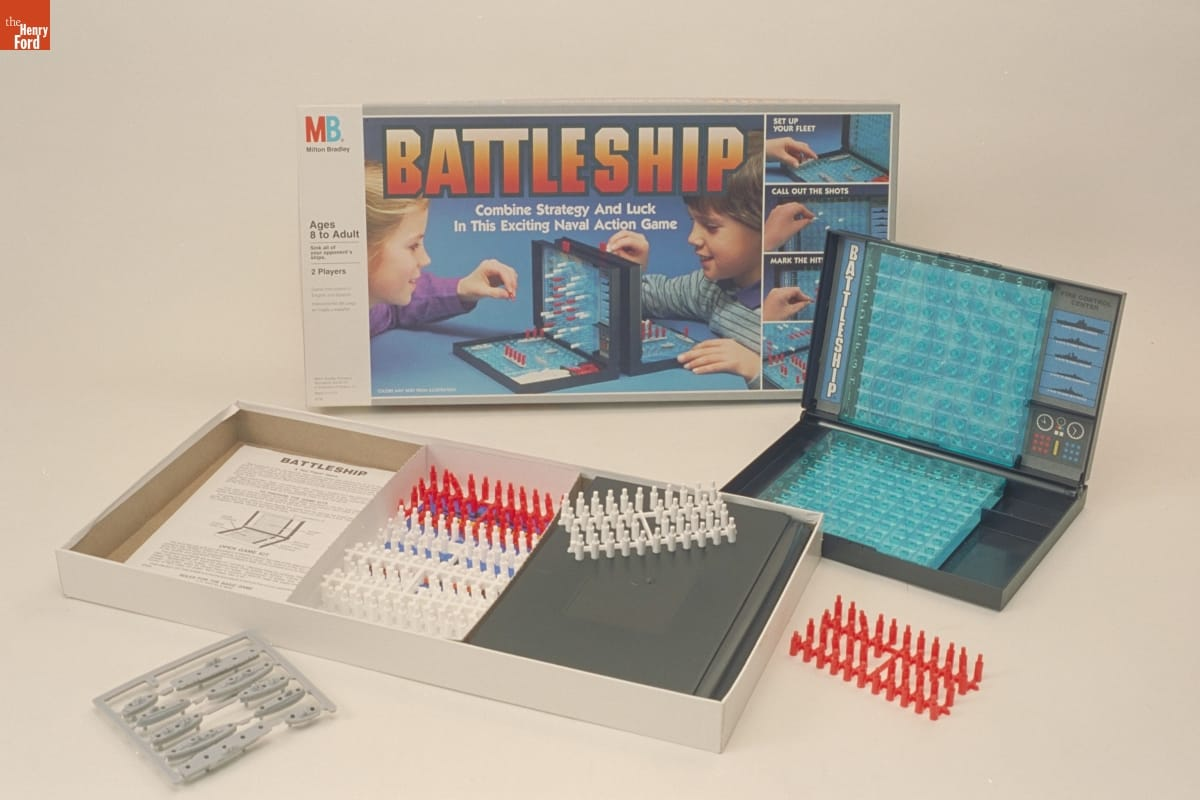
\includegraphics{imagenes/BattleShipOriginal.jpg}}
    \caption{Juego de mesa de hundir la flota. Año: 1980}
\end{figure}
\end{frame}


%%%%%%------Historia-----%%%%%%
\subsection{Historia}

\begin{frame}
  \frametitle{\insertsection}
  \framesubtitle{\hskip30pt \insertsubsection}

\begin{block}{Orígenes}
  \begin{itemize}
    \item\uncover<1->{Su posible origen está en el juego francés \textcolor{darkcerulean}{\em{L'Attaque}}\\ (publ. 	Hermance Edan, 1909)}
    \item\uncover<2->{La primera versión comercializada, \textcolor{orange}{\textit{Salvo}}, fue en 1931 por \textit{Starex Company.}}
    \item\uncover<3->{En 1967, \textcolor{blue}{Milton Bradley Company}, introduce una versión con tableros, barcos y otros elementos de plástico.}
    %\item En la actualidad, existen múltiples versiones digitales o en juegos de mesa.
  \end{itemize}
\end{block}

\end{frame}


\begin{frame}

  \begin{figure}
    \scalebox{0.55}{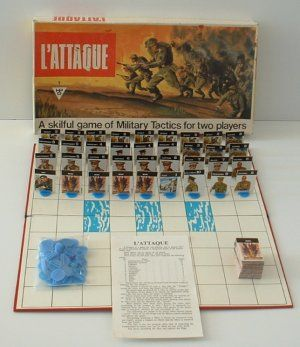
\includegraphics{imagenes/Lattaque.jpg}}
    \caption{Juego de mesa \em{L'Attaque}. Año: 1909}
  \end{figure}
\end{frame}

\begin{frame}

  \begin{figure}
    \scalebox{0.2}{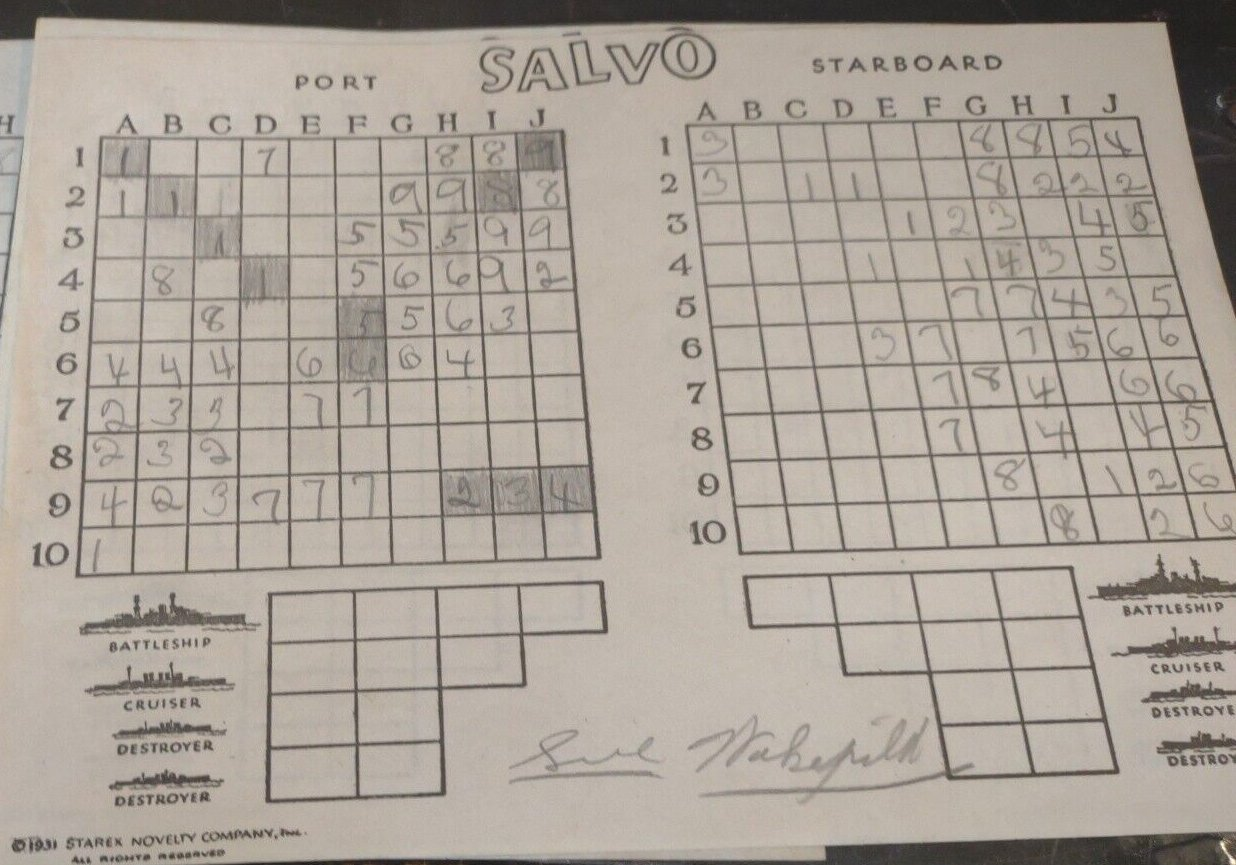
\includegraphics{imagenes/salvo2.jpg}}
    \caption{Juego de mesa \em{Salvo}. Año: 1931}
  \end{figure}
\end{frame}

\begin{frame}

  \begin{figure}
    \scalebox{0.6}{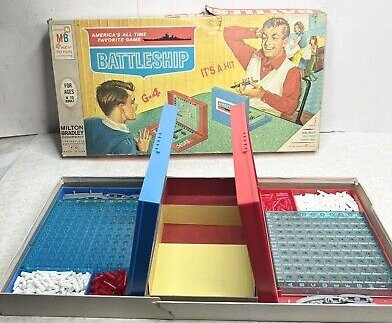
\includegraphics{imagenes/milton1967.jpg}}
    \caption{Juego de mesa \em{Battleship}. Año: 1967}
  \end{figure}
\end{frame}

\begin{frame}
  \frametitle{\insertsection}
  \framesubtitle{\hskip30pt \insertsubsection}

  \begin{block}{Evolución}

  \begin{itemize}
    \item\uncover<1->{En 1977, Milton lanza la primera versión computarizada: \textcolor{blue}{\textit{Electronic Battleship.}}}
    \item\uncover<2->{En 1984, \textcolor{orange}{Hasbro} adquiere Milton Bradley Company, y por tanto los derechos de \textit{Battleship}}
    \item\uncover<3->{La \textcolor{blue}{versión de Milton} es la que se ha expandido globalmente y la más conocida hasta hoy. }
    \item\uncover<4->{Se han creado múltiples variantes, desde juegos de mesa hasta digitales.}
   
  \end{itemize}
  \end{block}
\end{frame}

\begin{frame}

  \begin{figure}
    \scalebox{0.4}{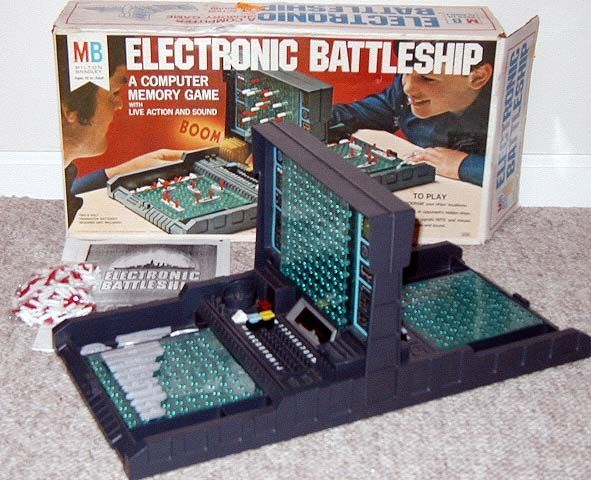
\includegraphics{imagenes/electronicBattleship.jpg}}
    \caption{Primera versión computarizada de \em{Battleship}. Año: 1977}
  \end{figure}
\end{frame}

\begin{frame}

  \begin{figure}
    \scalebox{0.23}{
\includegraphics{imagenes/battleshipHasbro.jpg}}
    \caption{Versión actual de \em{Battleship} de Hasbro.}
  \end{figure}
\end{frame}



\section{Descripción}


%%%%%%------Tableros-----%%%%%%
\subsection{Tableros}

\begin{frame}
    \frametitle{\insertsection}
    \framesubtitle{\hskip30pt \insertsubsection}

    \begin{block}{Tableros}
        \begin{itemize}
            \item\uncover<1->{Tamaño 10x10 casillas}
            \item\uncover<2->{Columnas identificadas con letras de la A - J}
            \item\uncover<3->{Filas numeradas del 1 al 10}
            \item\uncover<4->{Hay \textcolor{blue}{dos tableros:}}
                \begin{itemize}
                    \item\uncover<5->{\textbf{Tablero del jugador:} Donde el jugador coloca sus barcos y se registran
                    los disparos de la máquina.}
                    \item\uncover<6->{\textbf{Tablero del contrincante:} Donde la máquina coloca sus barcos y donde el jugador realiza sus disparos.}
                \end{itemize}
    \end{itemize}
    \end{block}
\end{frame}

\begin{frame}

    \begin{figure}
      \scalebox{0.34}{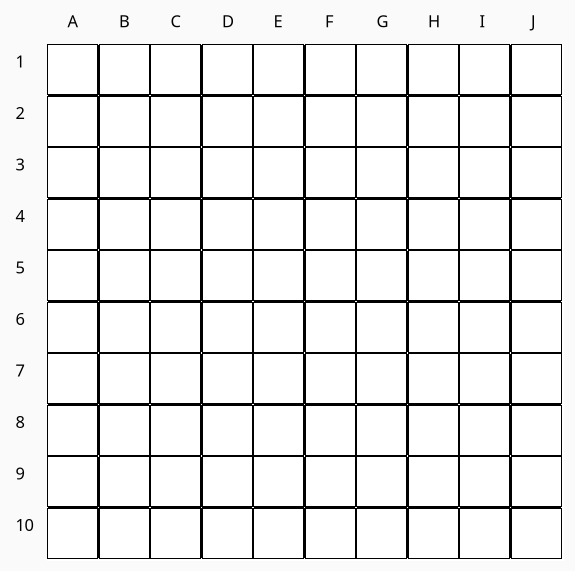
\includegraphics{imagenes/tablero.png}}
      \caption{Representación gráfica de un tablero}
    \end{figure}
\end{frame}


\subsection{Flota y restricciones en la colocación}

\begin{frame}
    \frametitle{\insertsection}
    \framesubtitle{\hskip30pt \insertsubsection}

    \begin{block}{Flota}
        \begin{itemize}
            \item\uncover<1->{1 x \textcolor{steelblue}{Portaaviones} de 5 casillas}
            \item\uncover<2->{1 x \textcolor{crimson}{Acorazado} de 4 casillas}
            \item\uncover<3->{ 2 x \textcolor{lightgreen}{Crucero} de 3 casillas}
            \item\uncover<4->{ 3 x \textcolor{darkkhaki}{Destructor} de 2 casillas}
            \item\uncover<5->{3 x \textcolor{navyblue}{Submarino} de 1 casilla}
        \end{itemize}
    \end{block}


\begin{figure}[h]
    \begin{columns}[c]
        
        \begin{column}{.2\textwidth}
            \centering
            \scalebox{0.4}{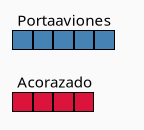
\includegraphics{imagenes/Barco1.png}}
        \end{column}

        \begin{column}{.2\textwidth}
            \centering
                \scalebox{0.34}{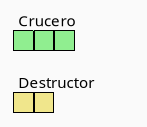
\includegraphics{imagenes/Barco2.png}}
        \end{column}

        \begin{column}{.2\textwidth}
            \centering
                \scalebox{0.34}{
\includegraphics{imagenes/Barco3.png}}
        \end{column}
   
    \end{columns}
    \caption{Representación de la flota}
\end{figure}

\end{frame}


\begin{frame}
    \begin{block}{Restricciones en la colocación de los barcos}
        \begin{itemize}
            \item\uncover<1->{ Se pueden colocar vertical u horizontalmente.}
            \item\uncover<2->{\textcolor{red}{No} se permiten casillas con barco \textcolor{red}{contiguas} (ni diagonalmente).}
        \end{itemize}
    \end{block}


\begin{figure}
    \begin{columns}[c]
        
        \begin{column}{.3\textwidth}
            \centering
            \scalebox{0.28}{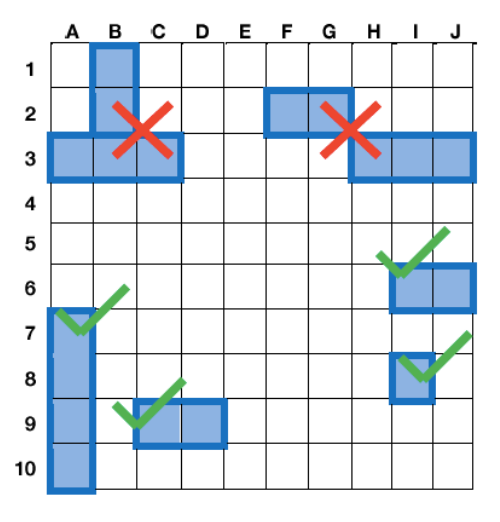
\includegraphics{imagenes/colocacionbarcos.png}}
        \end{column}
        \begin{column}{.3\textwidth}
            \centering
            \caption{Restricciones en la colocación}
        \end{column}
    \end{columns}
\end{figure}

\end{frame}


\subsection{Condición de victoria}

\begin{frame}
    \frametitle{\insertsection}
    \framesubtitle{\hskip30pt \insertsubsection}

    \begin{block}{Condición de victoria}
        Gana el primer jugador que \textcolor{blue}{hunda la flota} del contrincante.
    \end{block}
    
\end{frame}

\subsection{Contrincante}

\begin{frame}
    \frametitle{\insertsection}
    \framesubtitle{\hskip30pt \insertsubsection}

    \begin{block}{Contrincante}
        \begin{itemize}
            \item\uncover<1->{El único oponente será la \textcolor{blue}{CPU} (máquina).}
            \item\uncover<2->{Habrá tres tipos de algoritmos diferentes que podrá usar:}
            \begin{itemize}
                \item\uncover<3->{\textbf{Algoritmo aleatorio}}
                \item\uncover<4->{\textbf{Algoritmo Hunt/Target}}
                \item\uncover<5->{\textbf{Algoritmo Hunt/Target probabilístico}} 
            \end{itemize}
        \end{itemize}
    \end{block}
    
\end{frame}

\subsubsection{Algoritmo aleatorio}

\begin{frame}
    \frametitle{\insertsection}
    \framesubtitle{\hskip30pt \insertsubsection}

    \begin{block}{\textcolor{red}{Algoritmo aleatorio}}

        \begin{itemize}
            \item\uncover<1->{Realiza el disparo escogiendo una fila y una columna de forma aleatoria.}
            \item\uncover<2->{No escogerá casillas \textcolor{blue}{disparadas con anterioridad} o \textcolor{purple}{casillas contiguas} a barcos hundidos.}
        \end{itemize}
        
    \end{block}

    \begin{block}{Debilidades}
        \begin{itemize}
            \item\uncover<3->{Cuando un barco es alcanzado, el algoritmo no termina de hundirlo.}
            \item\uncover<4->{Recorre la mayoría de las casillas del tablero (muy ineficiente).}
        \end{itemize}
    \end{block}
\end{frame}

% \begin{frame}
%     \begin{figure}
%         \scalebox{0.34}{\includegraphics{imagenes/algoritmoAleatorio.gif}}
%         \caption{Representación gráfica de un tablero}
%       \end{figure}
% \end{frame}



\subsubsection{Algoritmo Hunt/Target}

\begin{frame}
    \frametitle{\insertsection}
    \framesubtitle{\hskip30pt \insertsubsection}

    \begin{block}{\textcolor{red}{Algoritmo Hunt/Target}}
        \begin{itemize}
            \item\uncover<1->{Usa \textcolor{red}{dos modos} (\textit{funciones}) alternos que usan una lista de objetivos conjuntamente para determinar la posición de un barco y hundirlo:}
            \begin{itemize}
                \item\uncover<2->{\textbf{Modo hunt} para buscar un objetivo}
                \item\uncover<3->{\textbf{Modo target} para hundir el barco}
            \end{itemize}
        \end{itemize}
    \end{block}
    
\end{frame}

\begin{frame}
    \frametitle{\insertsection}
    \framesubtitle{\hskip30pt \insertsubsection}

    \begin{block}{Modo Hunt}
        \begin{itemize}
            \item\uncover<1->{Dispara aleatoriamente una de las casillas del tablero que cumplan:}
            \begin{itemize}
                \item\uncover<2->{\textcolor{red}{no} disparadas con anterioridad ni contiguas a barcos hundidos.}
                \item\uncover<3->{\textcolor{blue}{pariedad par} y \textcolor{purple}{espacio} disponible para el barco de menor longitud sin hundir.}
            \end{itemize}
            \item\uncover<4->{Si el disparo es sobre un \textcolor{red}{barco}, se crea una \textcolor{darkcerulean}{lista con sus casillas vecinas} N - S - E - O}
        \end{itemize}
        
    \end{block}
\end{frame}

\begin{frame}
    \begin{block}{Pariedad par}
        Que casillas (mínimas) debe contener parte de un barco colocado de cualquier forma en el tablero.   
    \end{block}

    \begin{block}{Nota}
        Se aplica para el \textcolor{blue}{barco de menor longitud sin hundir} para garantizar tocar a todos los barcos en menos disparos.
    \end{block}
        
\end{frame}

\begin{frame}
    \begin{figure}
        \begin{columns}[c]
            
            \begin{column}{.5\textwidth}
                \centering
                \scalebox{0.30}{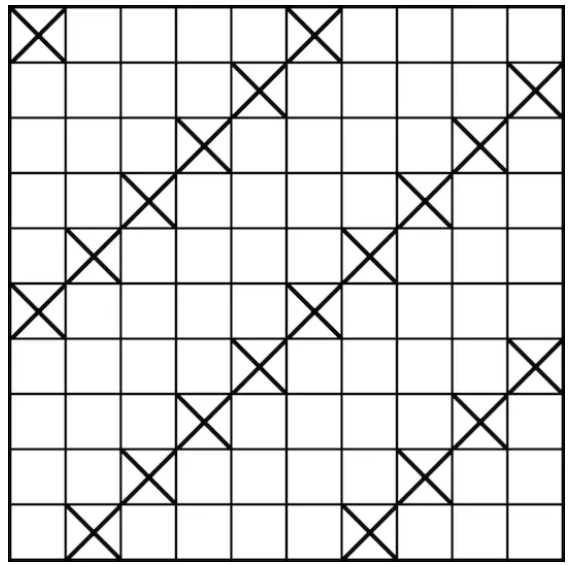
\includegraphics{imagenes/pariedad.png}}
            \end{column}
            \begin{column}{.3\textwidth}
                \centering
                \caption{Patrón de disparo para un barco de 5 casillas}
            \end{column}
        \end{columns}
    \end{figure}
\end{frame}

\begin{frame}
    \begin{block}{Espacio disponible}
        La casilla seleccionada debe contener al menos \textcolor{blue}{una dirección con suficientes casillas vacías} para albergar el barco
        de menor longitud sin hundir.
    \end{block}

\end{frame}

\begin{frame}
    \frametitle{\insertsection}
    \framesubtitle{\hskip30pt \insertsubsection}

    \begin{block}{Modo target}
        \begin{itemize}
            \item\uncover<1->{Dispara a las casillas de la \textcolor{blue}{lista objetivos} para precisar la \textcolor{red}{orientación} del barco:}
            \begin{itemize}
                \item\uncover<2->{Si el disparo es en la misma fila: \textcolor{purple}{horizontal}.}
                \item\uncover<3->{Si el disparo es en la misma columna: \textcolor{blue}{navyblue}.}
            \end{itemize}
            \item\uncover<4->{Una vez precisada la orientación, por cada acierto, se añade a la lista de objetivos la \textcolor{blue}{siguiente casilla} de la misma fila (horizontal) o de la misma columna (vertical).}
            \item\uncover<5->{Una vez que el barco es \textcolor{red}{hundido}, se vuelve al modo hunt para repetir el proceso.}
        \end{itemize}
    \end{block}

\end{frame}

\begin{frame}
    
    \begin{block}{Notas sobre la \textcolor{blue}{lista de objetivos}}
        \begin{itemize}
            \item\uncover<1->{Hay que \textit{barajarla} al principio para que los barcos verticales no tengan desventaja.}
            \item\uncover<2->{Es necesaria para \textcolor{green}{guardar los objetivos} después de un cambio de turno, o retroceder si el disparo no ha sido en los extremos}
            \item\uncover<3->{\textcolor{red}{Solo} contiene casillas no disparadas ni contiguas a barcos hundidos y dentro de los límites del tablero.}
        \end{itemize}
        
    \end{block}
\end{frame}

\begin{frame}
    \begin{block}{Fortalezas}
        \begin{itemize}
            \item\uncover<1->{Cuando un barco es alcanzado es hundido.}
            \item\uncover<2->{Se realizan menos disparos (es más eficiente).}
            \item\uncover<3->{Durante la evolución de la partida, el algoritmo es más rápido en hundir barcos.}
        \end{itemize}
    \end{block}
    \uncover<3->{\begin{block}{Debilidades}
        \begin{itemize}
            \item\uncover<3->{Todavía sigue usando aleatoriedad.}
            \item\uncover<4->{Necesita una lista de objetivos.}
            \item\uncover<5->{Al existir el barco de una casilla, en la mayoría de partidas el modo hunt no se beneficia de sus filtros.}
        \end{itemize}
    \end{block}}
\end{frame}

\subsubsection{Algoritmo Hunt/Target probabilístico}

\begin{frame}
    \frametitle{\insertsection}
    \framesubtitle{\hskip30pt \insertsubsection}

    \begin{block}{\textcolor{red}{Algoritmo Hunt/Target probabilístico}}
        \begin{itemize}
            \item\uncover<1->{Usa la \textcolor{blue}{misma idea} de los dos \textit{modos} que el algoritmo Hunt/Target normal.}
            \item\uncover<2->{\textcolor{red}{Mejora} el modo hunt y modo target para eliminar la \textit{aleatoriedad}.}
            \item\uncover<3->{Se mantiene el uso de la lista de objetivos}
            \item\uncover<4->{Se usan las \textit{\textbf{funciones de densidad de probabilidad}} para tomar las decisiones.}
        \end{itemize}
    \end{block}

    \uncover<5->{\begin{block}{Nota}
        Se puede usar una versión de este algoritmo sin lista de objetivos. Todas las decisiones serían
        tomadas con probabilidad.

    \end{block}}
    
\end{frame}

\begin{frame}
    \frametitle{\insertsection}
    \framesubtitle{\hskip30pt \insertsubsection}

    \begin{block}{Funciones de densidad de probabilidad} 
        \begin{itemize}
            \item\uncover<1->{Se considera que en el centro del tablero habrá más \textcolor{red}{densidad de barcos.}}
            \item\uncover<2->{Por cada casilla que haya un barco se asigna un \textbf{\textit{peso}.}}
            \item\uncover<3->{Se calculan todas las posibles posiciones en todas las casillas con todos los barcos \textcolor{purple}{(\textit{superposición})}}
            \item\uncover<4->{Al sumarse los pesos por cada posible variación en cada casilla, se obtiene una \textcolor{blue}{matriz de probabilidades.}}
        \end{itemize}    
    \end{block}


\end{frame}

\begin{frame}
    \begin{figure}
        \scalebox{0.4}{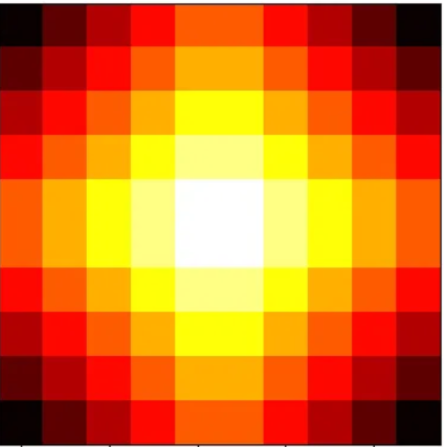
\includegraphics{imagenes/mapaCalorPortaaviones.png}}
        \caption{Ejemplo de representación de la matriz de probabilidad en un mapa de calor para un portaaviones}
      \end{figure}
\end{frame}

\begin{frame}
    \begin{figure}
        \scalebox{0.4}{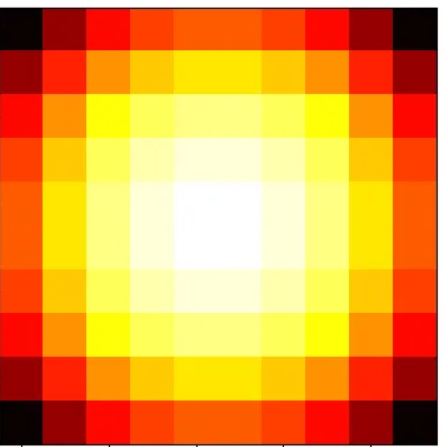
\includegraphics{imagenes/flotaMapa.png}}
        \caption{Ejemplo de representación de la matriz de probabilidad en un mapa de calor con todos los barcos}
      \end{figure}
\end{frame}

\begin{frame}
    \frametitle{\insertsection}
    \framesubtitle{\hskip30pt \insertsubsection}

    \begin{block}{Modo Hunt}
        \begin{itemize}
            \item\uncover<1->{Al principio, la \textcolor{blue}{matriz de probabilidades} es actualizada.}
            \begin{itemize}
                \item\uncover<2->{Las casillas disparadas o contiguas a barcos hundidos tendrán \textcolor{red}{probabilidad 0.}}
                \item\uncover<3->{Al calcular todas las posibles posiciones de los barcos, estos \textcolor{red}{no} pueden superponerse en casillas disparadas o contiguas a barcos hundidos.}
            \end{itemize}
            \item\uncover<4->{El objetivo será aquella casilla con \textcolor{blue}{mayor probabilidad.}}
            \begin{itemize}
                \item\uncover<5->{Si el disparo \textcolor{red}{falla}, se volverá a intentar con la siguiente mayor en el siguiente turno.}
                \item\uncover<6->{Si el disparo \textcolor{blue}{acierta}, se añaden las casillas vecinas a la lista de objetivos y se pasa el relevo al \textcolor{purple}{modo target.}}
            \end{itemize}
            
        \end{itemize}
    \end{block}
    
\end{frame}

\begin{frame}
    \frametitle{\insertsection}
    \framesubtitle{\hskip30pt \insertsubsection}

    \begin{block}{Modo Target}
        \begin{itemize}
            \item\uncover<1->{Usa la misma lógica que el modo target anterior.}
            \item\uncover<2->{La matriz de probabilidades es usada para decidir en que orden disparar sobre las casillas vecinas.}
            \item\uncover<3->{Si el disparo es sobre agua, se vuelven a calcular las probabilidades para elegir la casilla con mayor probabilidad.}
            \item\uncover<4->{Cuando la orientación es elegida, se actúa de la forma anterior (no se usa la matriz de probabilidades).}
        \end{itemize}
    \end{block}
    
\end{frame}

\begin{frame}
    \begin{block}{Fortalezas}
        \begin{itemize}
            \item\uncover<1->{Si la flota es colocada aleatoriamente (densidad alta en el centro), el \textcolor{red}{algoritmo es muy eficaz}}
            \item\uncover<2->{Permite ajustar la estrategia cambiando artificialmente los pesos según se desee}
            \item\uncover<3->{\textcolor{blue}{Fácilmente adaptable} para algoritmos más avanzados (Machine Learning)}
        \end{itemize}
    \end{block}
    \uncover<3->{\begin{block}{Debilidades}
        \begin{itemize}
            \item\uncover<4->{Usa una \textcolor{red}{estructura de datos auxiliar} extra (matriz de probabilidades).}
            \item\uncover<5->{Supone un gasto mayor en recursos en calcular cada vez la matriz de probabilidades.}
            \item\uncover<6->{Es \textcolor{red}{débil} si los barcos son colocados alejados del centro.}
        \end{itemize}
    \end{block}}
\end{frame}

\section{Descripción modular del código}

\subsection{Estructuras de datos}

\subsubsection{Barcos}

\begin{frame}
    \frametitle{\insertsection}
    \framesubtitle{\hskip30pt \insertsubsection}

    \begin{block}{Barcos}
        \begin{itemize}
            \item Vectores de vectores (matrices)
            \item Cada fila representa a un \textcolor{blue}{tipo de barco} (portaaviones, acorazado, crucero, destructor o submarino).
            \item Las columnas son los siguientes campos por cada tipo de barco:
            \begin{itemize}
                \item ID: número para identificar el tipo de barco
                \item Nombre: cadena con el nombre del tipo
                \item Número de barcos (sin colocar): número de barcos en total
                \item Tamaño del barco: número de casillas que ocupan
                \item Color: cadena con el color que son representados
                \item Barcos restantes (sin hundir): número de barcos a flote
                \item Lista con el tamaño de cada barco: controla el tamaño de cada barco
            \end{itemize}
        \end{itemize}
    \end{block}
\end{frame}


\subsubsection{Tableros/flota}

\begin{frame}
    \frametitle{\insertsection}
    \framesubtitle{\hskip30pt \insertsubsection}

    \begin{block}{Tableros/flota}
        \begin{itemize}
            \item Vectores de vectores (matrices)
            \item Representan \textcolor{blue}{el tablero de cada jugador.}
            \item Guardan la información de la colocación de los barcos. 
            \item El agua es representada con un 0 mientras que cada barco es una lista:
            \begin{itemize}
                \item ID: número del tipo de barco.
                \item SubID: número que identifica al barco dentro de su mismo tipo.
                \item Posición proa: sublista con las coordenadas de la casilla dónde se sitúa la proa del barco.
                \item Tamaño del barco: número que indica el número de casillas que ocupa
                \item Orientación: booleano que indica su posición.
            \end{itemize}
        \end{itemize}
    \end{block}
\end{frame}


\subsubsection{Mapas de disparo}

 \begin{frame}
     \frametitle{\insertsection}
     \framesubtitle{\hskip30pt \insertsubsection}
     \begin{block}{Mapas de disparos}
        \begin{itemize}
             \item Vectores de vectores (matrices)
             \item Representan los \textcolor{blue}{disparos que ha realizado el jugador} en una casilla del tablero del contrincante.
             \item Mismo tamaño que los tableros.
             \item Contienen la siguiente información:
             \begin{itemize}
                 \item 0: casilla sin descubrir.
                 \item 1: casilla de barco descubierta
                 \item -1: casilla de agua descubierta
                 \item -2: exclusión alrededor de barco hundido (solo es usado por los algoritmos de la máquina)
             \end{itemize}
        \end{itemize}
     \end{block}
 \end{frame}

 \subsubsection{Matriz de probabilidades}

 \begin{frame}
     \frametitle{\insertsection}
     \framesubtitle{\hskip30pt \insertsubsection}
     \begin{block}{Matriz de probabilidades}
         \begin{itemize}
             \item Vectores de vectores (matrices)
             \item Representa la \textcolor{blue}{probabilidad de cada casilla de contener un barco.}
             \item Mismo tamaño que los tableros.
             \item Solo es usado por el algoritmo Hunt/Target probabilístico
             \item Contiene por cada casilla la suma de los pesos.
         \end{itemize}
     \end{block}
 \end{frame}



\subsection{Estructura de archivos}

\begin{frame}
    \frametitle{\insertsection}
    \framesubtitle{\hskip30pt \insertsubsection}

    \begin{block}{}
        \renewcommand\DTstyle{\sffamily}
        \begin{small}
            
        
        \dirtree{%
        .1 \textbf{HundirFlota/}.
        .2 + archivo-tableros/ \\Archivador de tableros (generado).
        .2 + gui/ - Elementos de la interfaz.
        .3 botones.rkt.
        .3 canvas.rkt.
        .3 dialogos.rkt.
        .3 mensajes.rkt.
        .3 opciones.rkt.
        .3 paneles.rkt.
        .3 temporizadores.rkt.
        .3 textos.rkt.
        .3 ventana.rkt.
        }
    \end{small}
    \end{block}
\end{frame}

\begin{frame}
    \begin{block}{}
        \renewcommand\DTstyle{\sffamily}
        \begin{small}
            
        
        \dirtree{%
        .1 \textbf{HundirFlota/}.
        .2 + gui/.
        .3 + funcionesCallback - Funciones de los elementos gráficos.
        .4 callbackBotones.rkt.
        .4 callbackCanvas.rkt.
        .4 callbackDialogos.rkt.
        .4 callbackOpciones.rkt.
        .4 callbackTemporizadores.rkt.
        .4 callbackVentanas.rkt.
        }
    \end{small}
    \end{block}
\end{frame}


\begin{frame}
    \begin{block}{}
        \renewcommand\DTstyle{\sffamily}
        \begin{small}
            
        
        \dirtree{%
        .1 \textbf{HundirFlota/}.
        .2 funciones.rkt \\ Funciones variadas.
        .2 funcionesGUI.rkt.\\ Funciones variadas de GUI.
        .2 turno.rkt \\ Función cambio de turno.    
        }
    \end{small}
    \end{block}
\end{frame}

\begin{frame}
    \begin{block}{}
        \renewcommand\DTstyle{\sffamily}
        \begin{small}
            
        
        \dirtree{%
        .1 \textbf{HundirFlota/}.
        .2 funcionesLimpiar.rkt \\ Limpieza de canvases.
        .2 funcionesColocar.rkt \\ Colocación de barcos y su lógica.
        .2 funcionesDibujar.rkt \\ Dibujado en canvas.
        .2 funcionesDisparar.rkt \\ Lógica de disparar.
        .2 funcionesGenerar.rkt \\ Generación aleatoria en la colocación de barcos.
        .2 funcionesLogica.rkt \\ Lógica del juego.     
        }
    \end{small}
    \end{block}
\end{frame}

\begin{frame}
    \begin{block}{}
        \renewcommand\DTstyle{\sffamily}
        \begin{small}
            
        
        \dirtree{%
        .1 \textbf{HundirFlota/}.
        .2 + imagenes/ \\ Recursos gráficos.
        .2 + ayuda/ \\ Recursos de ayuda.
        .2 main.rkt \\ Programa principal.
        .2 estructuras.rkt \\ Estructuras principales.
        .2 macros.rkt \\ Macros globales.
        }
    \end{small}
    \end{block}
\end{frame}



\section{Resultados}


\begin{frame}
     \begin{figure}
         \scalebox{0.60}{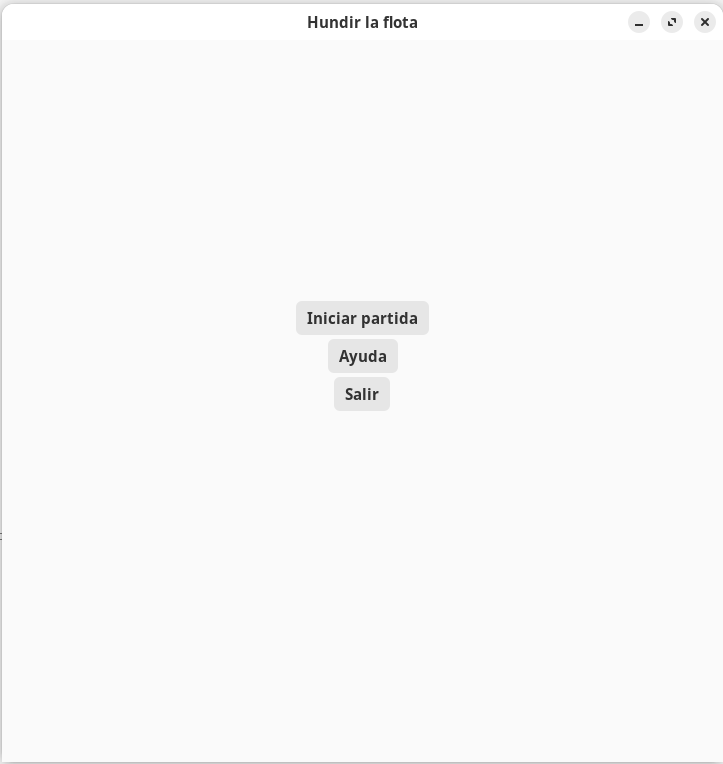
\includegraphics[width = \textwidth]{imagenes/resultados/inicio.png}}
         \caption{Menú de inicio de la aplicación}
       \end{figure}
\end{frame}

\begin{frame}
    \begin{columns}
        \column{\dimexpr\paperwidth-10pt}
        \begin{figure}
            \scalebox{1}{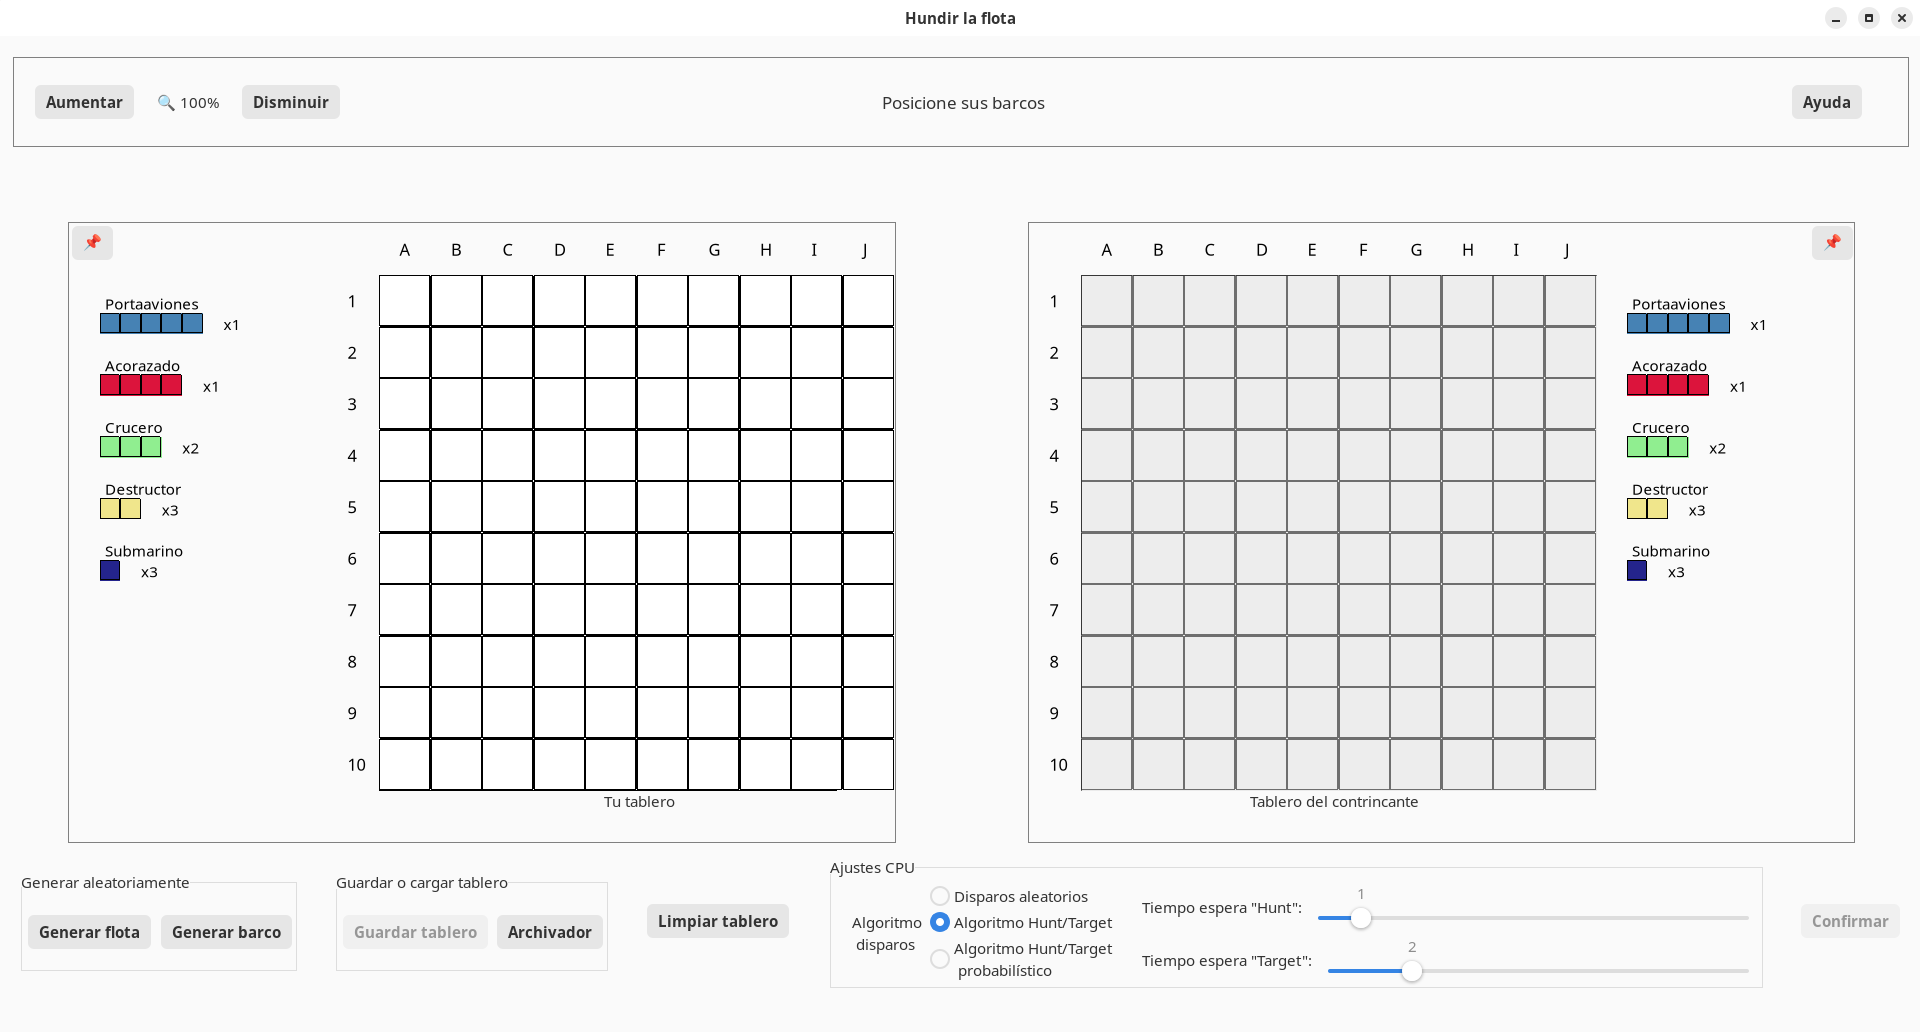
\includegraphics[width = \textwidth]{imagenes/resultados/principal.png}}
            \caption{Pantalla principal de la aplicación}
          \end{figure}
      \end{columns}
\end{frame}

\begin{frame}
    \begin{columns}
        \column{\dimexpr\paperwidth-10pt}
        \begin{figure}
            \scalebox{1}{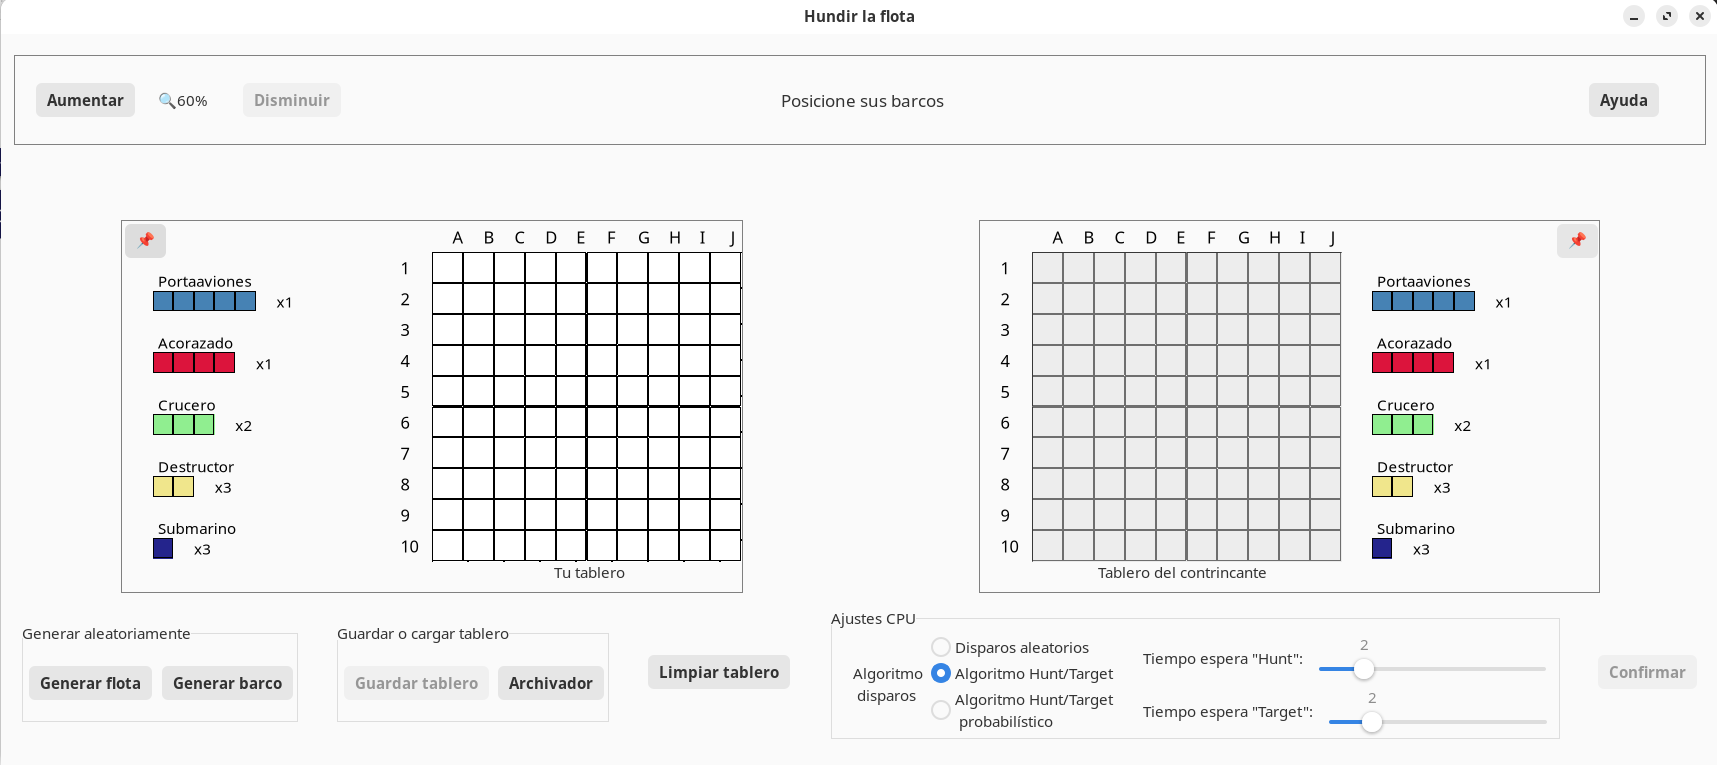
\includegraphics[width = \textwidth]{imagenes/resultados/disminuir.png}}
            \caption{Disminuir el tamaño de la interfaz}
          \end{figure}
      \end{columns}
\end{frame}

\begin{frame}
    \begin{columns}
        \column{\dimexpr\paperwidth-10pt}
        \begin{figure}
            \scalebox{1}{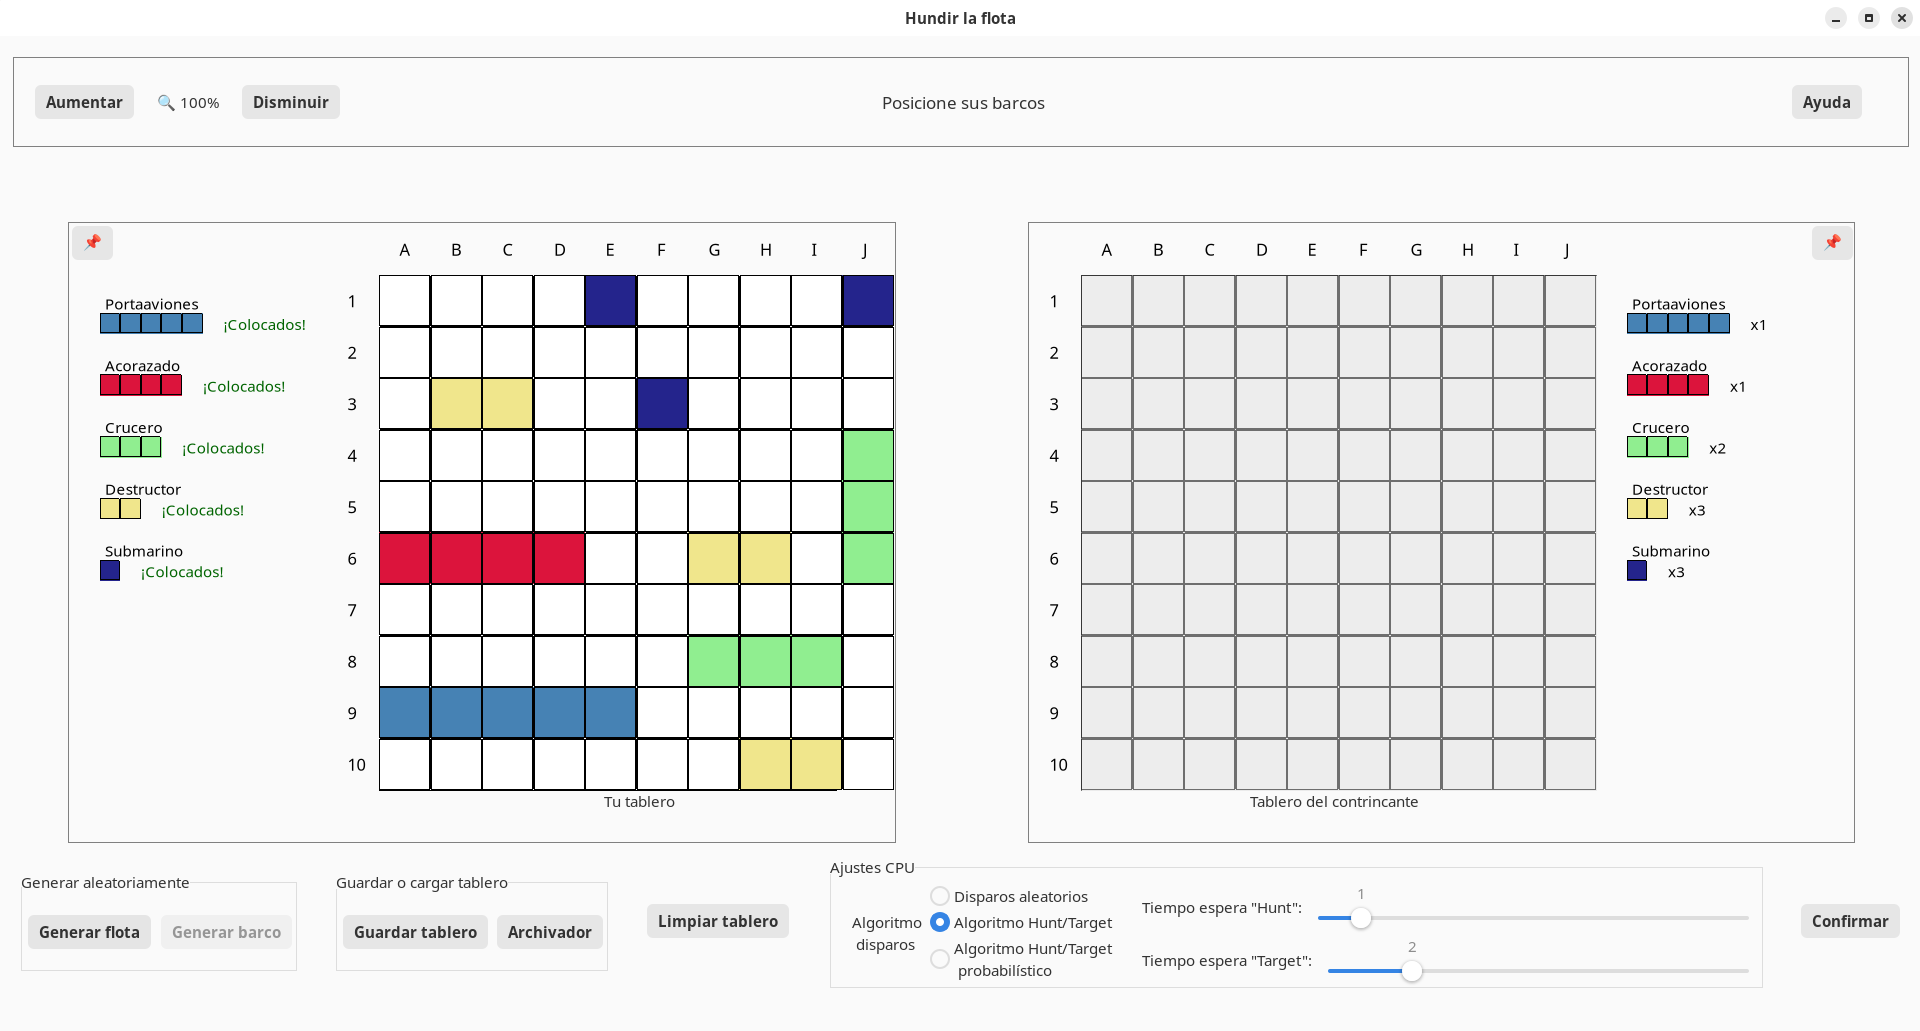
\includegraphics[width = \textwidth]{imagenes/resultados/colocacionAleatoria.png}}
            \caption{Ejemplo de colocación de los barcos aleatoria}
          \end{figure}
      \end{columns} 
\end{frame}

\begin{frame}
    \begin{columns}
        \column{\dimexpr\paperwidth-10pt}
        \begin{figure}
            \scalebox{1}{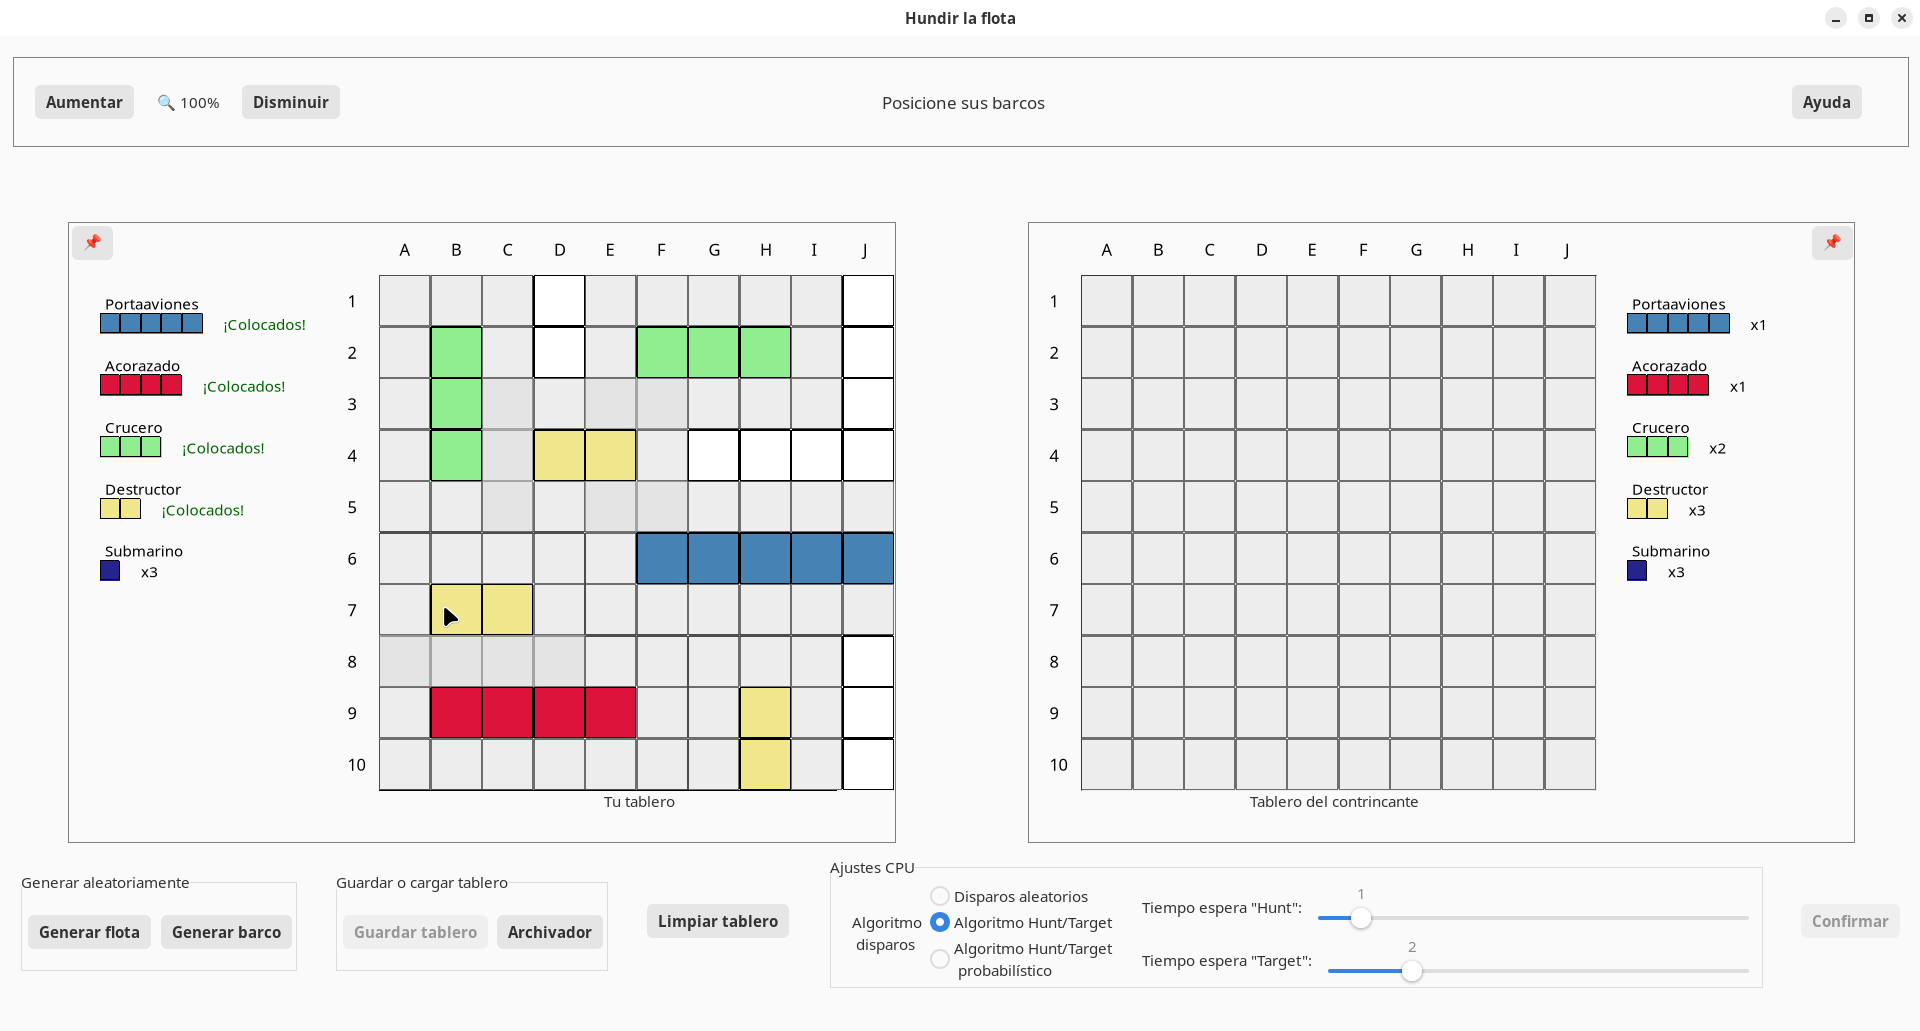
\includegraphics[width = \textwidth]{imagenes/resultados/colocacionManual.png}}
            \caption{Ejemplo de colocación de los barcos manual}
          \end{figure}
      \end{columns}   
\end{frame}


\begin{frame}
    \begin{columns}
        \column{\dimexpr\paperwidth-10pt}
        \begin{figure}
            \scalebox{1}{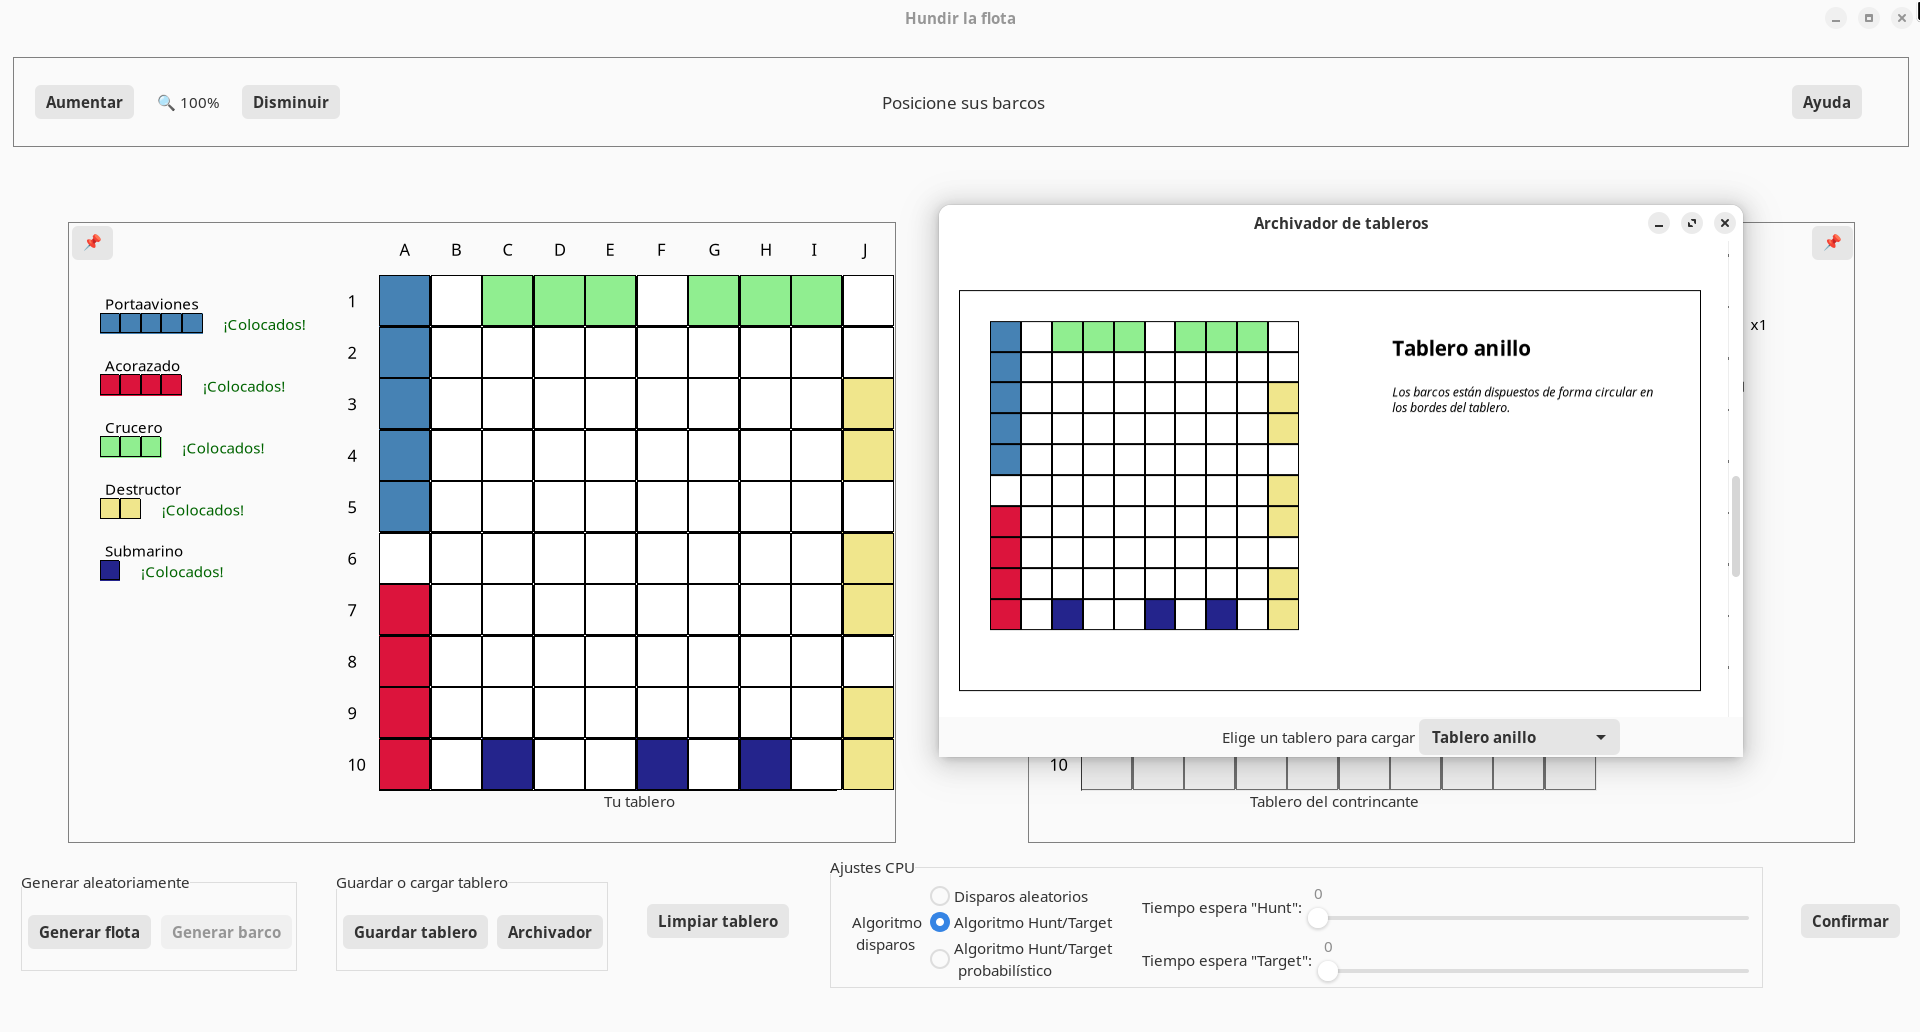
\includegraphics[width = \textwidth]{imagenes/resultados/cargar.png}}
            \caption{Uso del archivador}
          \end{figure}
      \end{columns}
\end{frame}

\begin{frame}
    \begin{columns}
        \column{\dimexpr\paperwidth-10pt}
        \begin{figure}
            \scalebox{1}{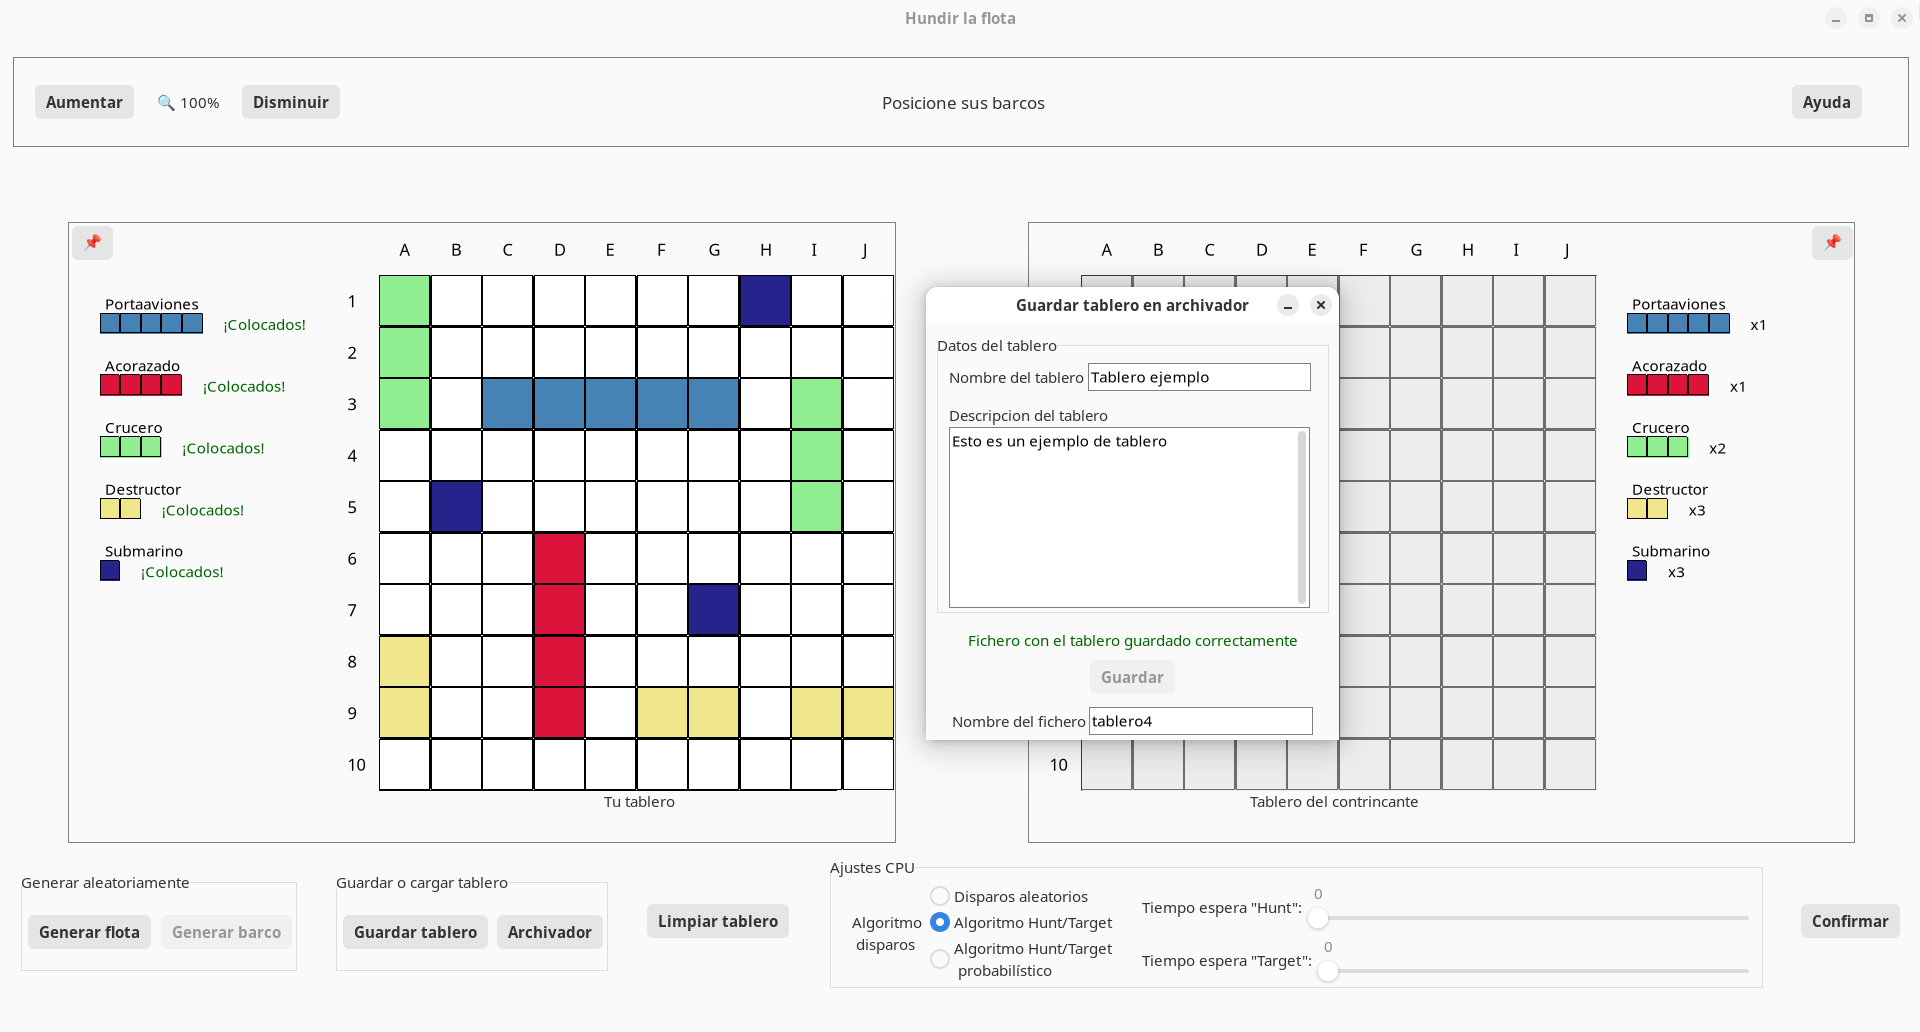
\includegraphics[width = \textwidth]{imagenes/resultados/guardar.png}}
            \caption{Guardar un tablero en el archivador}
          \end{figure}
      \end{columns}
\end{frame}

\begin{frame}
    \begin{columns}
        \column{\dimexpr\paperwidth-10pt}
        \begin{figure}
            \scalebox{1}{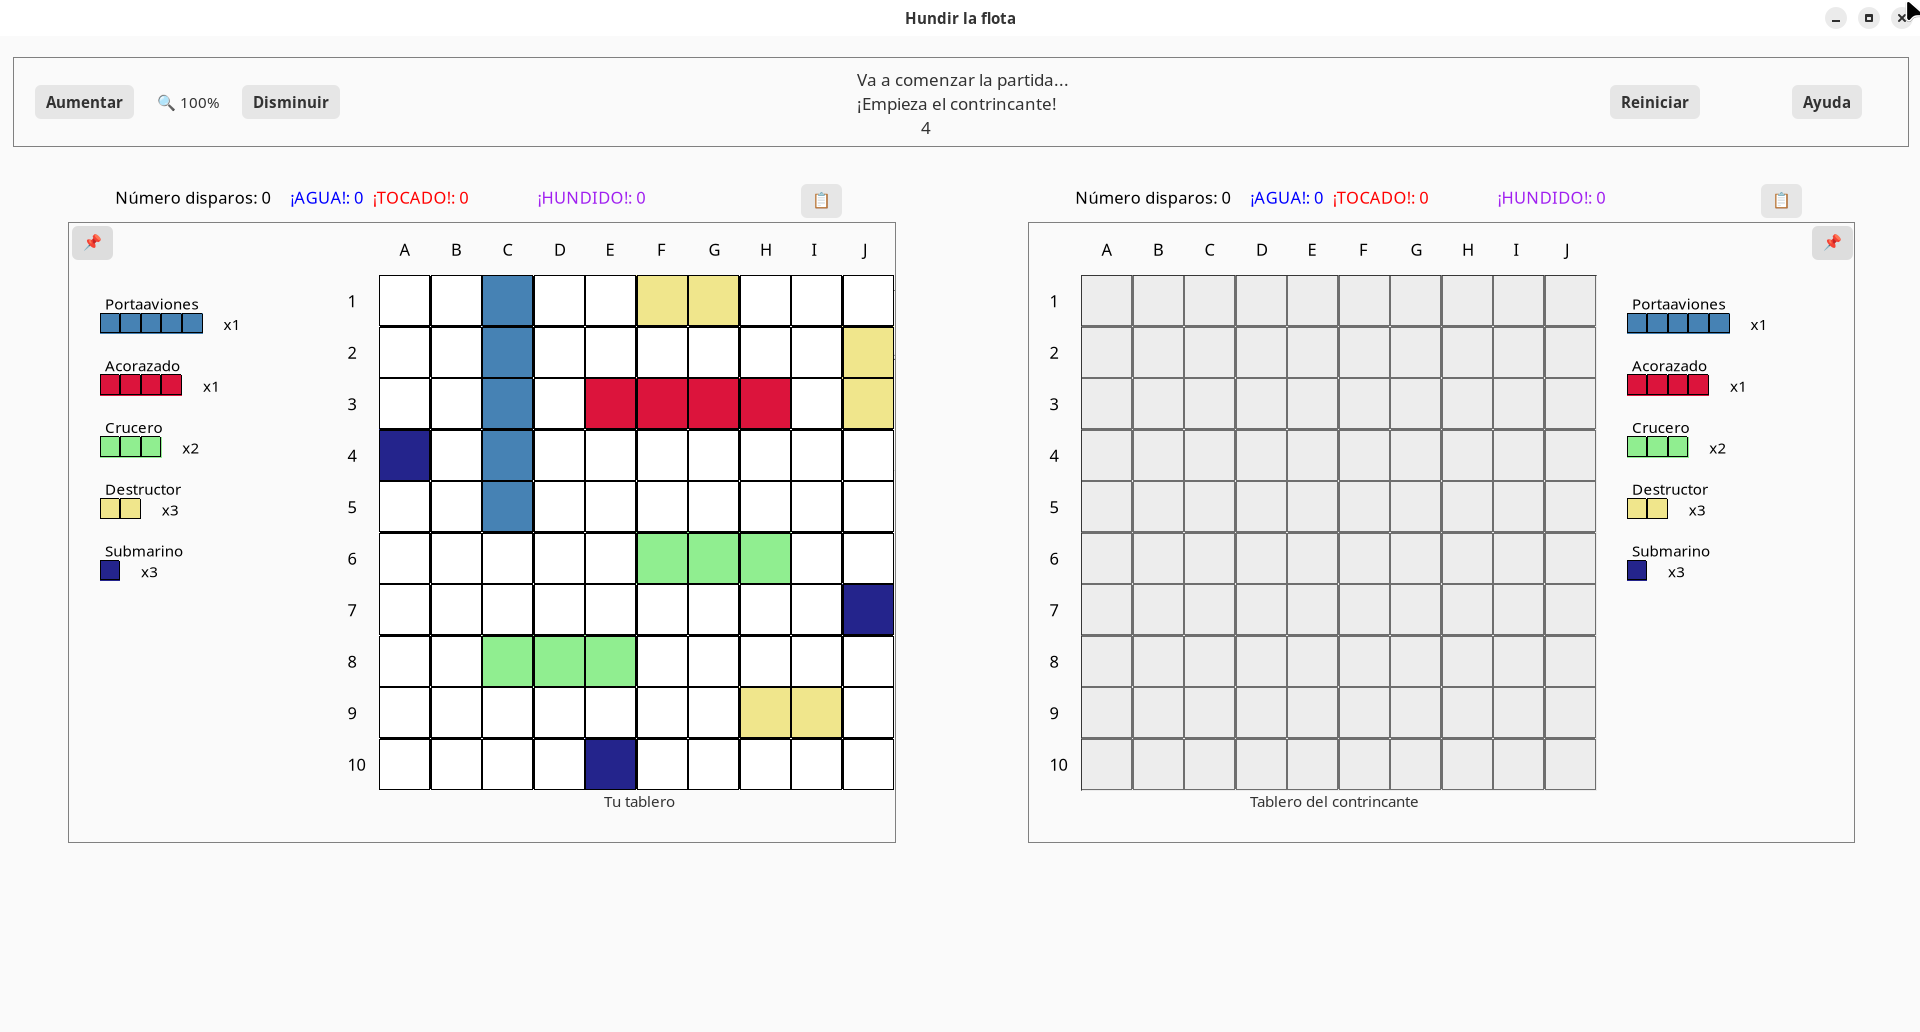
\includegraphics[width = \textwidth]{imagenes/resultados/partida.png}}
            \caption{Inicio de partida}
          \end{figure}
      \end{columns}
\end{frame}

\begin{frame}
    \begin{columns}
        \column{\dimexpr\paperwidth-10pt}
        \begin{figure}
            \scalebox{1}{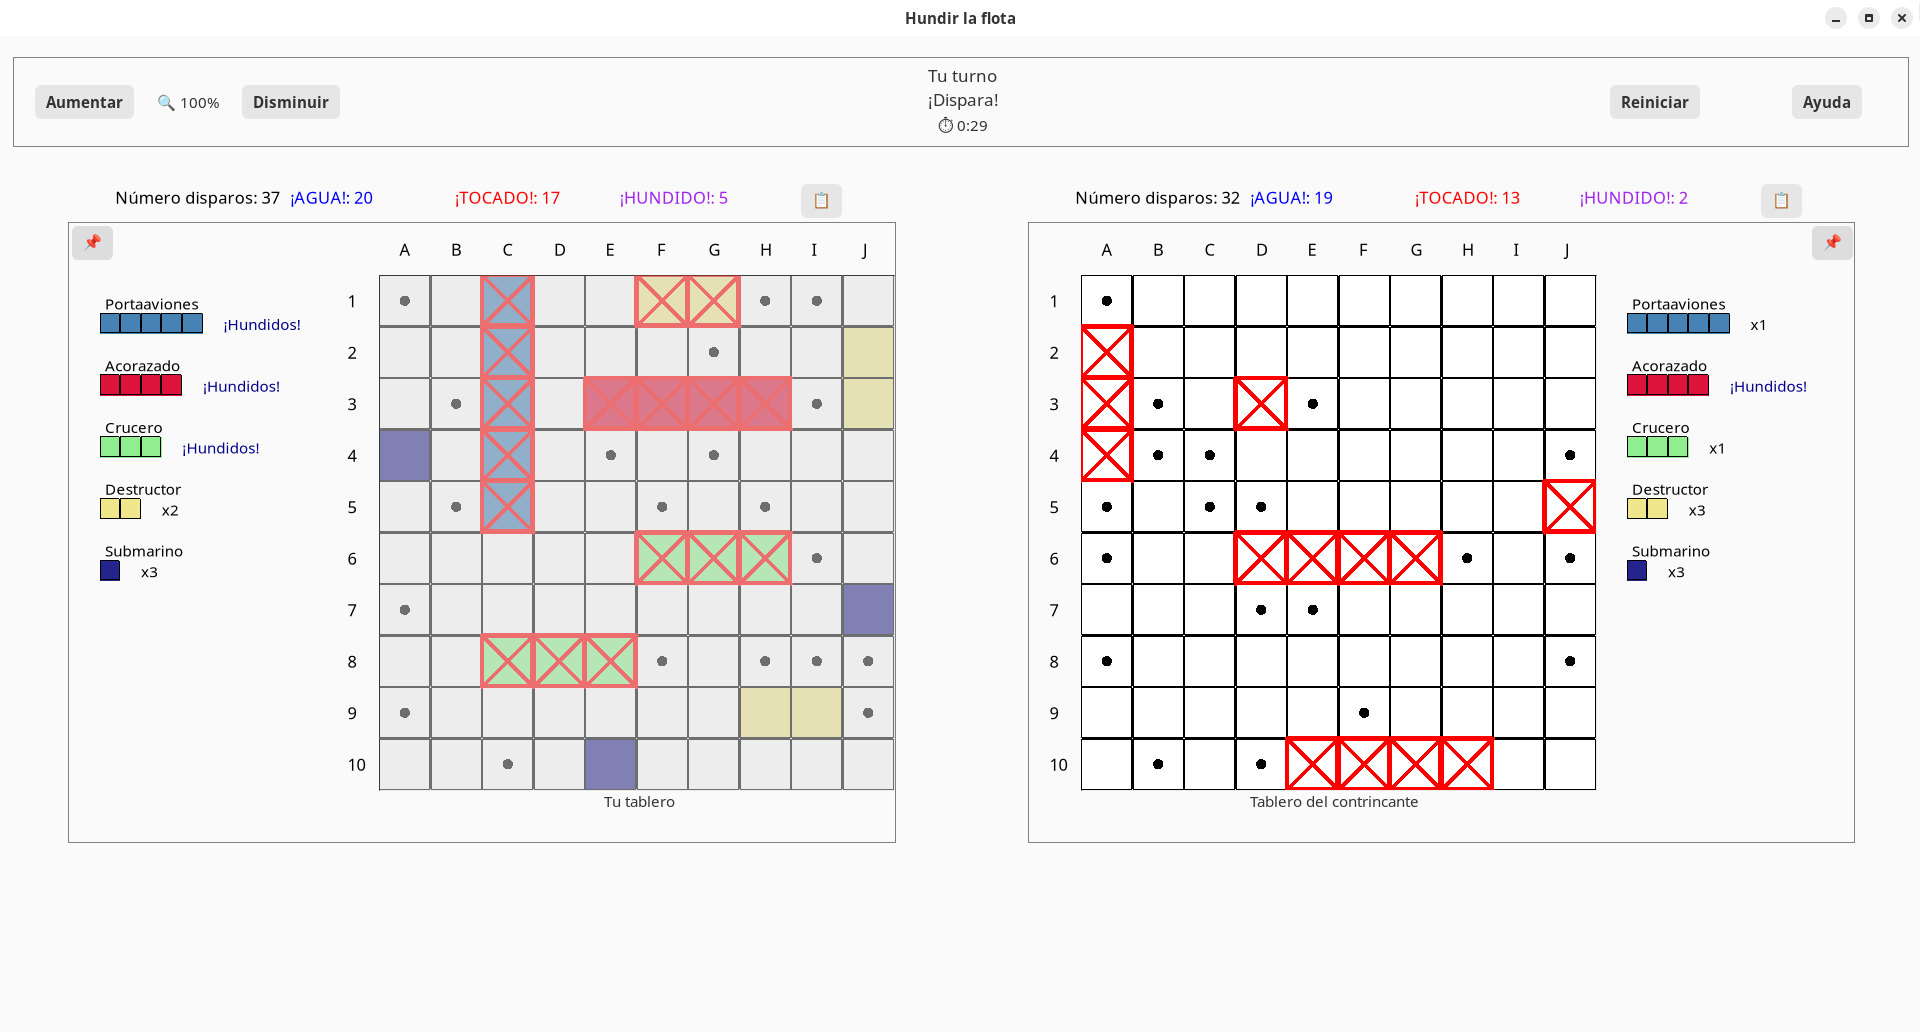
\includegraphics[width = \textwidth]{imagenes/resultados/turnoJugador.png}}
            \caption{Turno del jugador}
          \end{figure}
      \end{columns}
\end{frame}

\begin{frame}
    \begin{columns}
        \column{\dimexpr\paperwidth-10pt}
        \begin{figure}
            \scalebox{1}{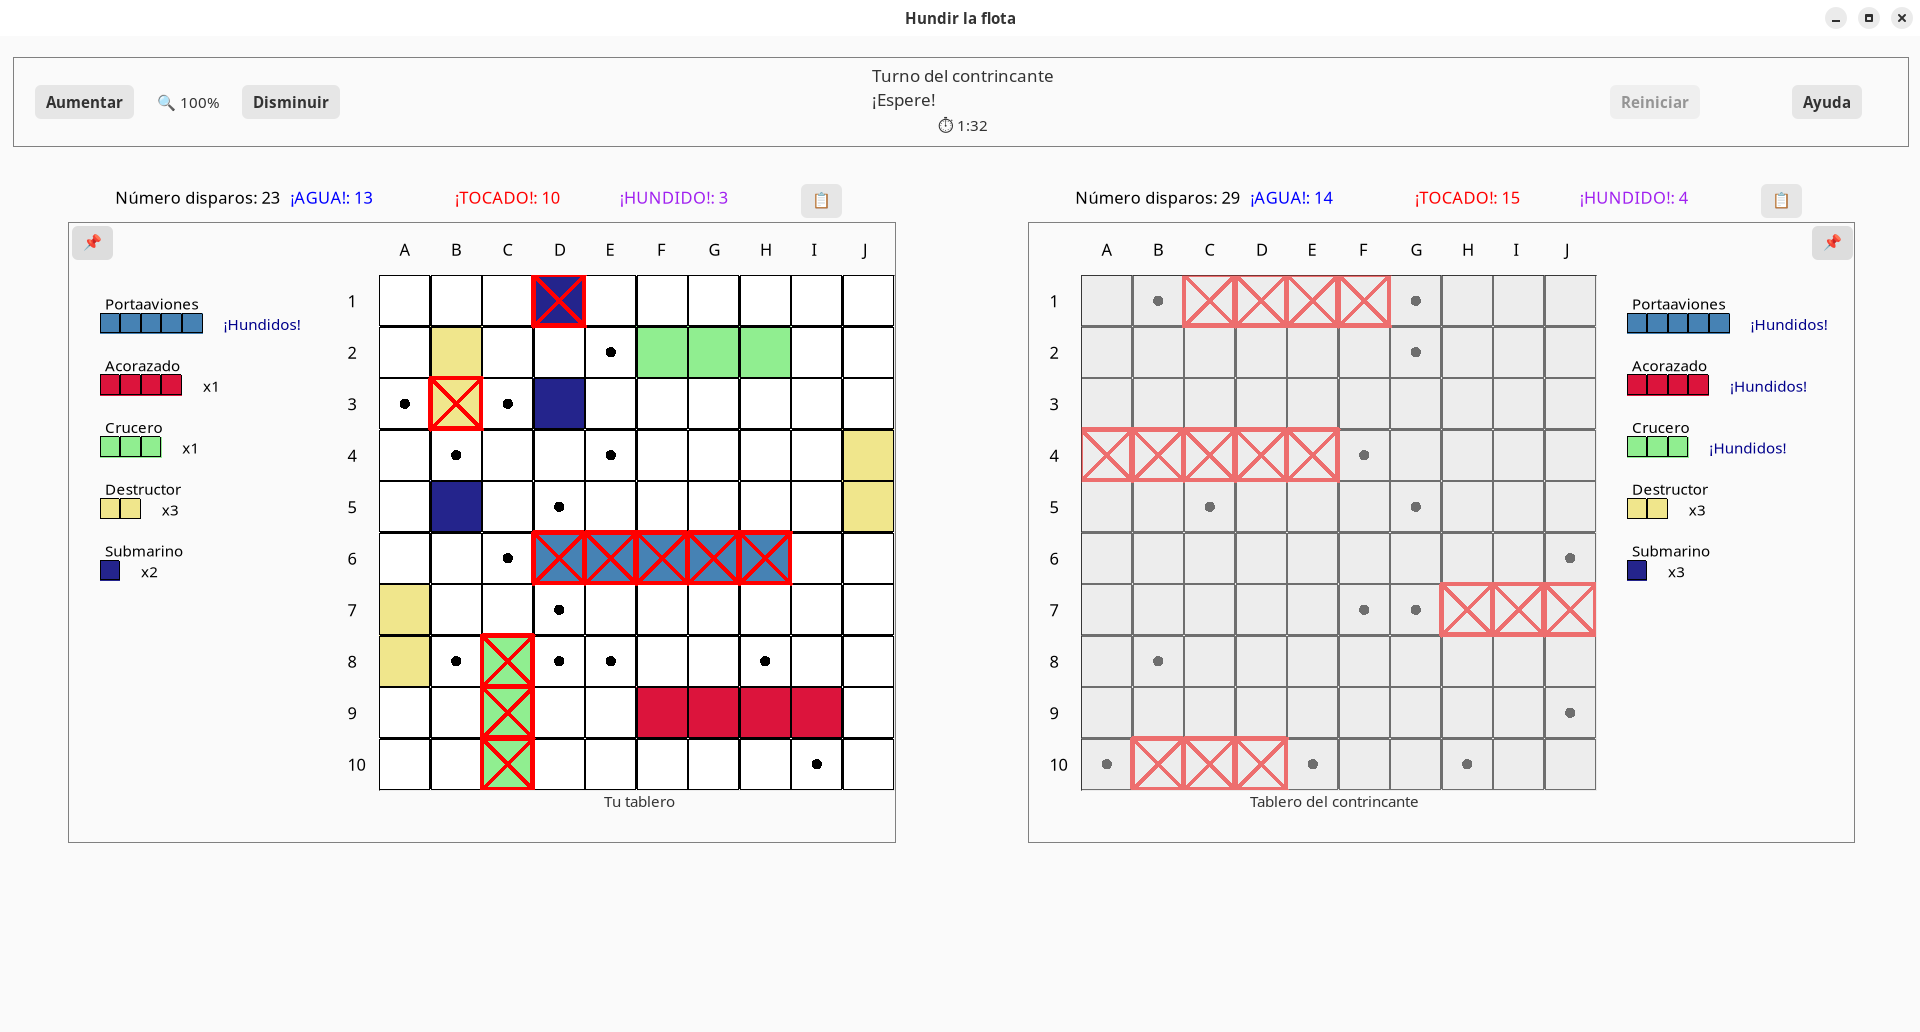
\includegraphics[width = \textwidth]{imagenes/resultados/turnoCPU.png}}
            \caption{Turno de la máquina (\textit{CPU})}
          \end{figure}
      \end{columns}
\end{frame}


\begin{frame}
    \begin{columns}
        \column{\dimexpr\paperwidth-10pt}
        \begin{figure}
            \scalebox{1}{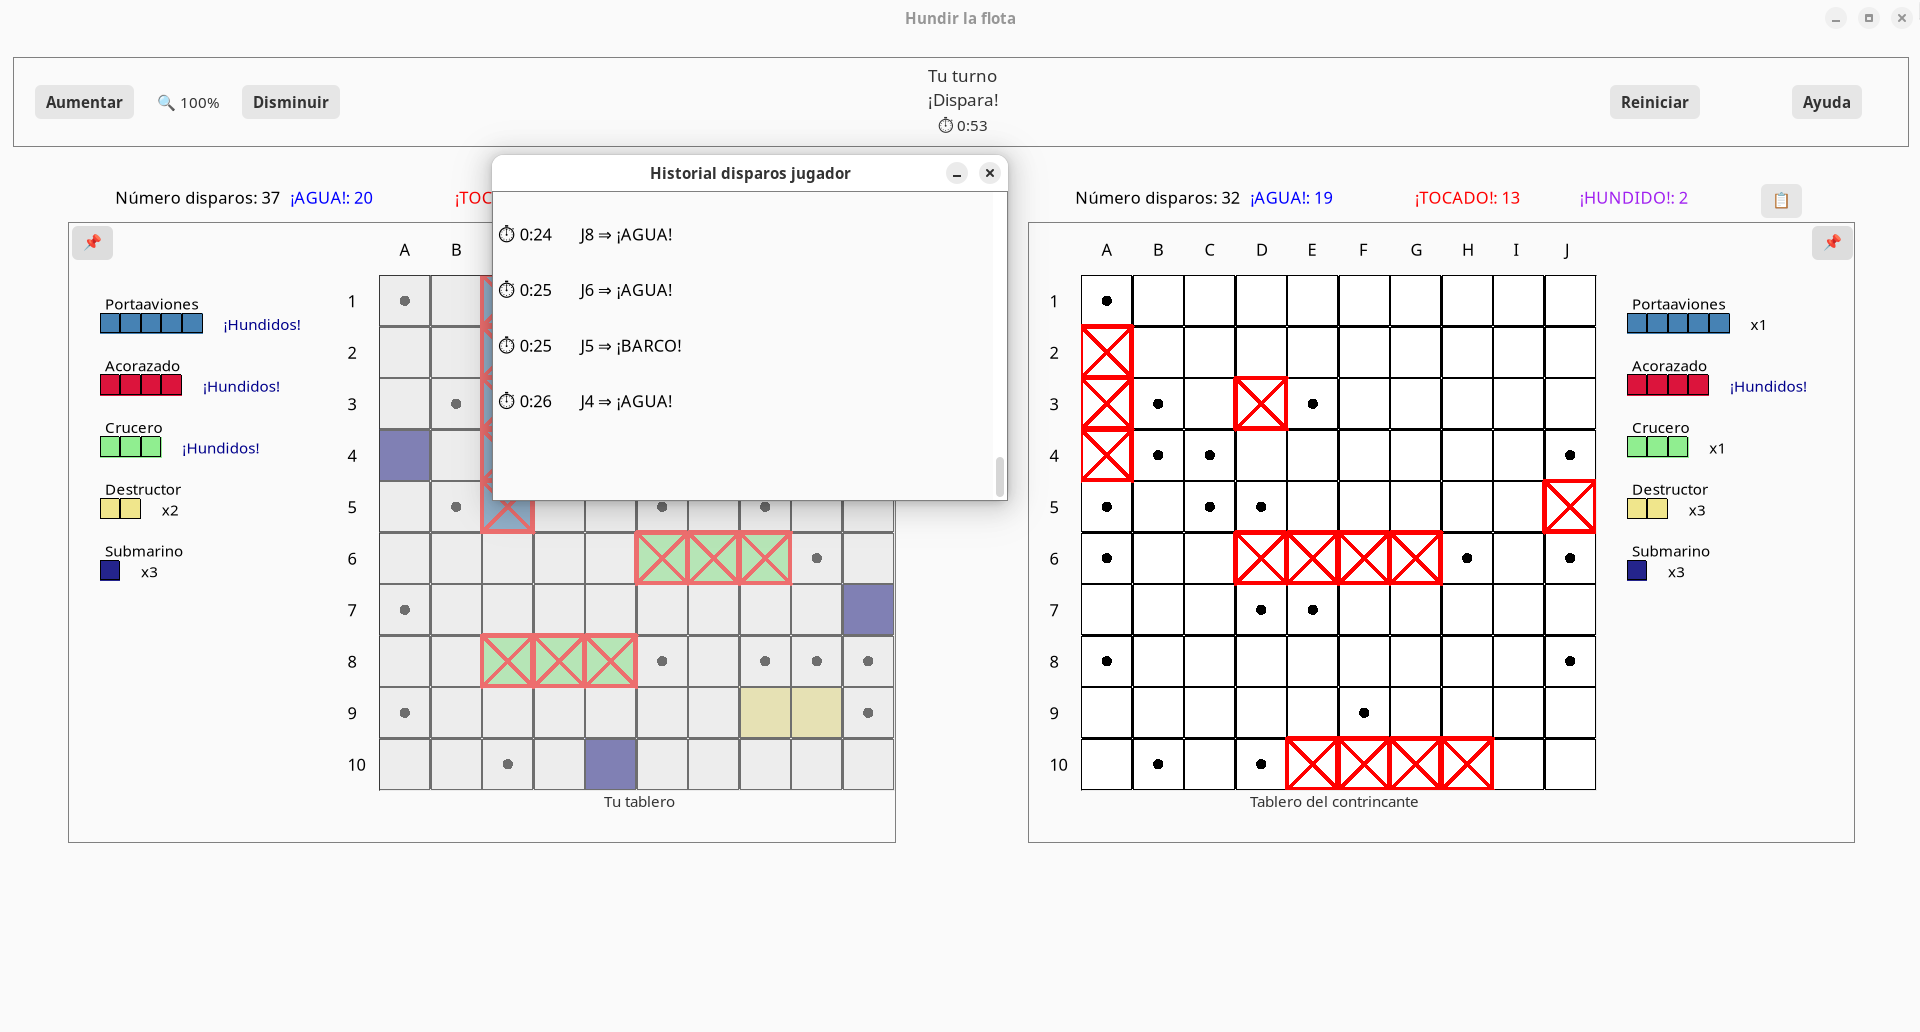
\includegraphics[width = \textwidth]{imagenes/resultados/historial.png}}
            \caption{Uso del historial de disparos}
          \end{figure}
      \end{columns}
\end{frame}


\begin{frame}
    \begin{columns}
        \column{\dimexpr\paperwidth-10pt}
        \begin{figure}
            \scalebox{1}{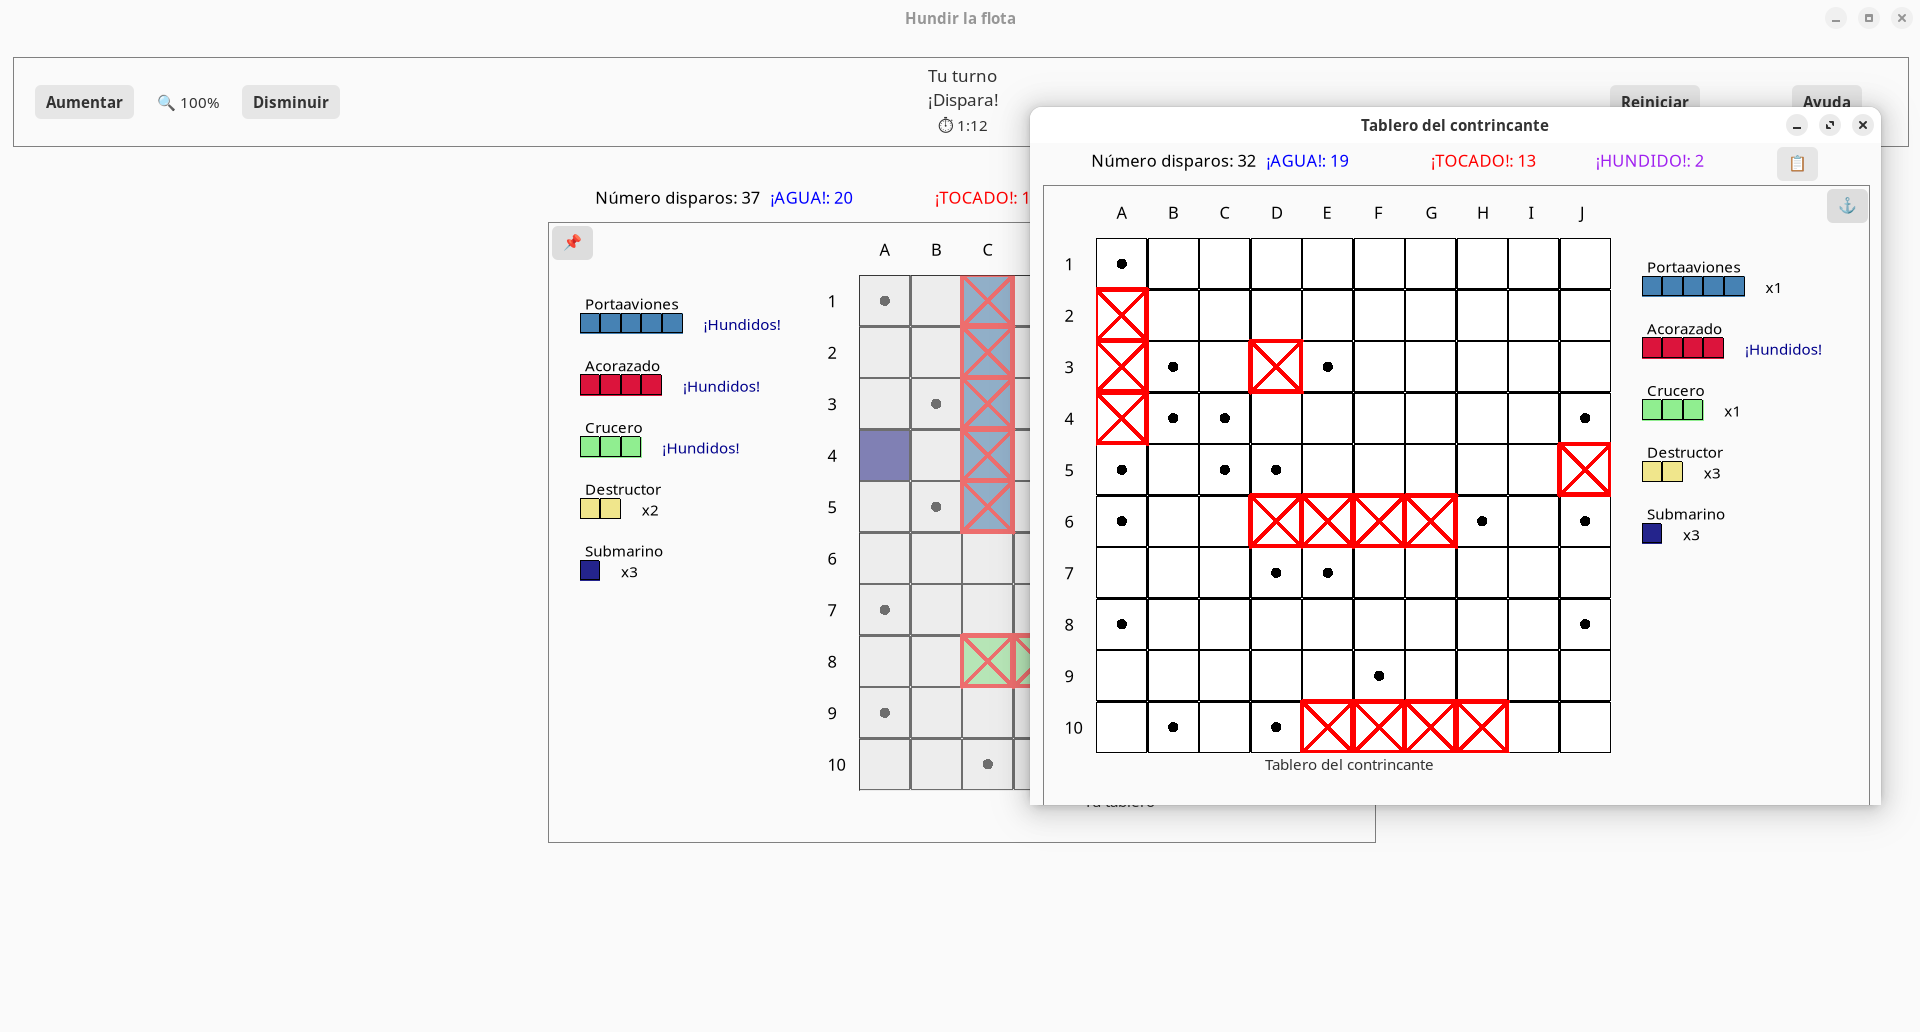
\includegraphics[width = \textwidth]{imagenes/resultados/desanclar.png}}
            \caption{Desanclar un tablero}
          \end{figure}
      \end{columns}
\end{frame}

\begin{frame}
    \begin{columns}
        \column{\dimexpr\paperwidth-10pt}
        \begin{figure}
            \scalebox{1}{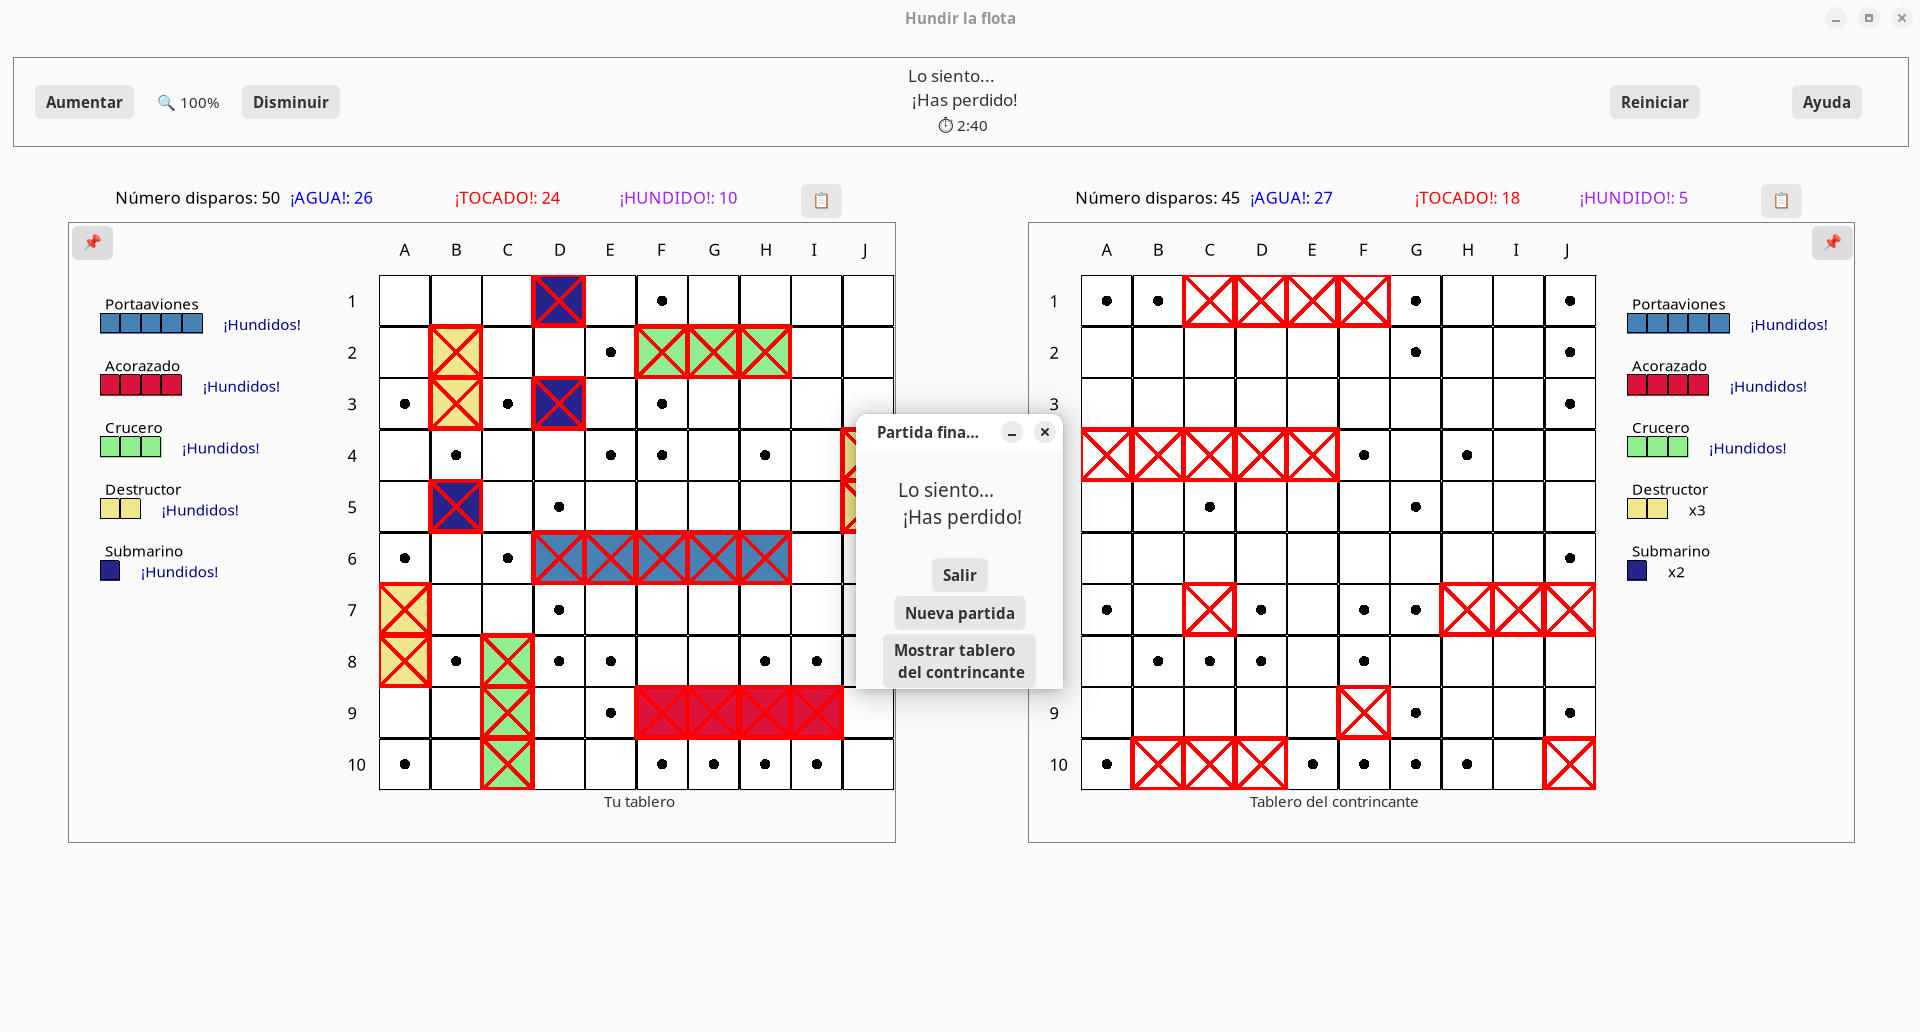
\includegraphics[width = \textwidth]{imagenes/resultados/final.png}}
            \caption{Final de una partida}
          \end{figure}
      \end{columns}
\end{frame}

\begin{frame}
    \begin{columns}
        \column{\dimexpr\paperwidth-10pt}
        \begin{figure}
            \scalebox{1}{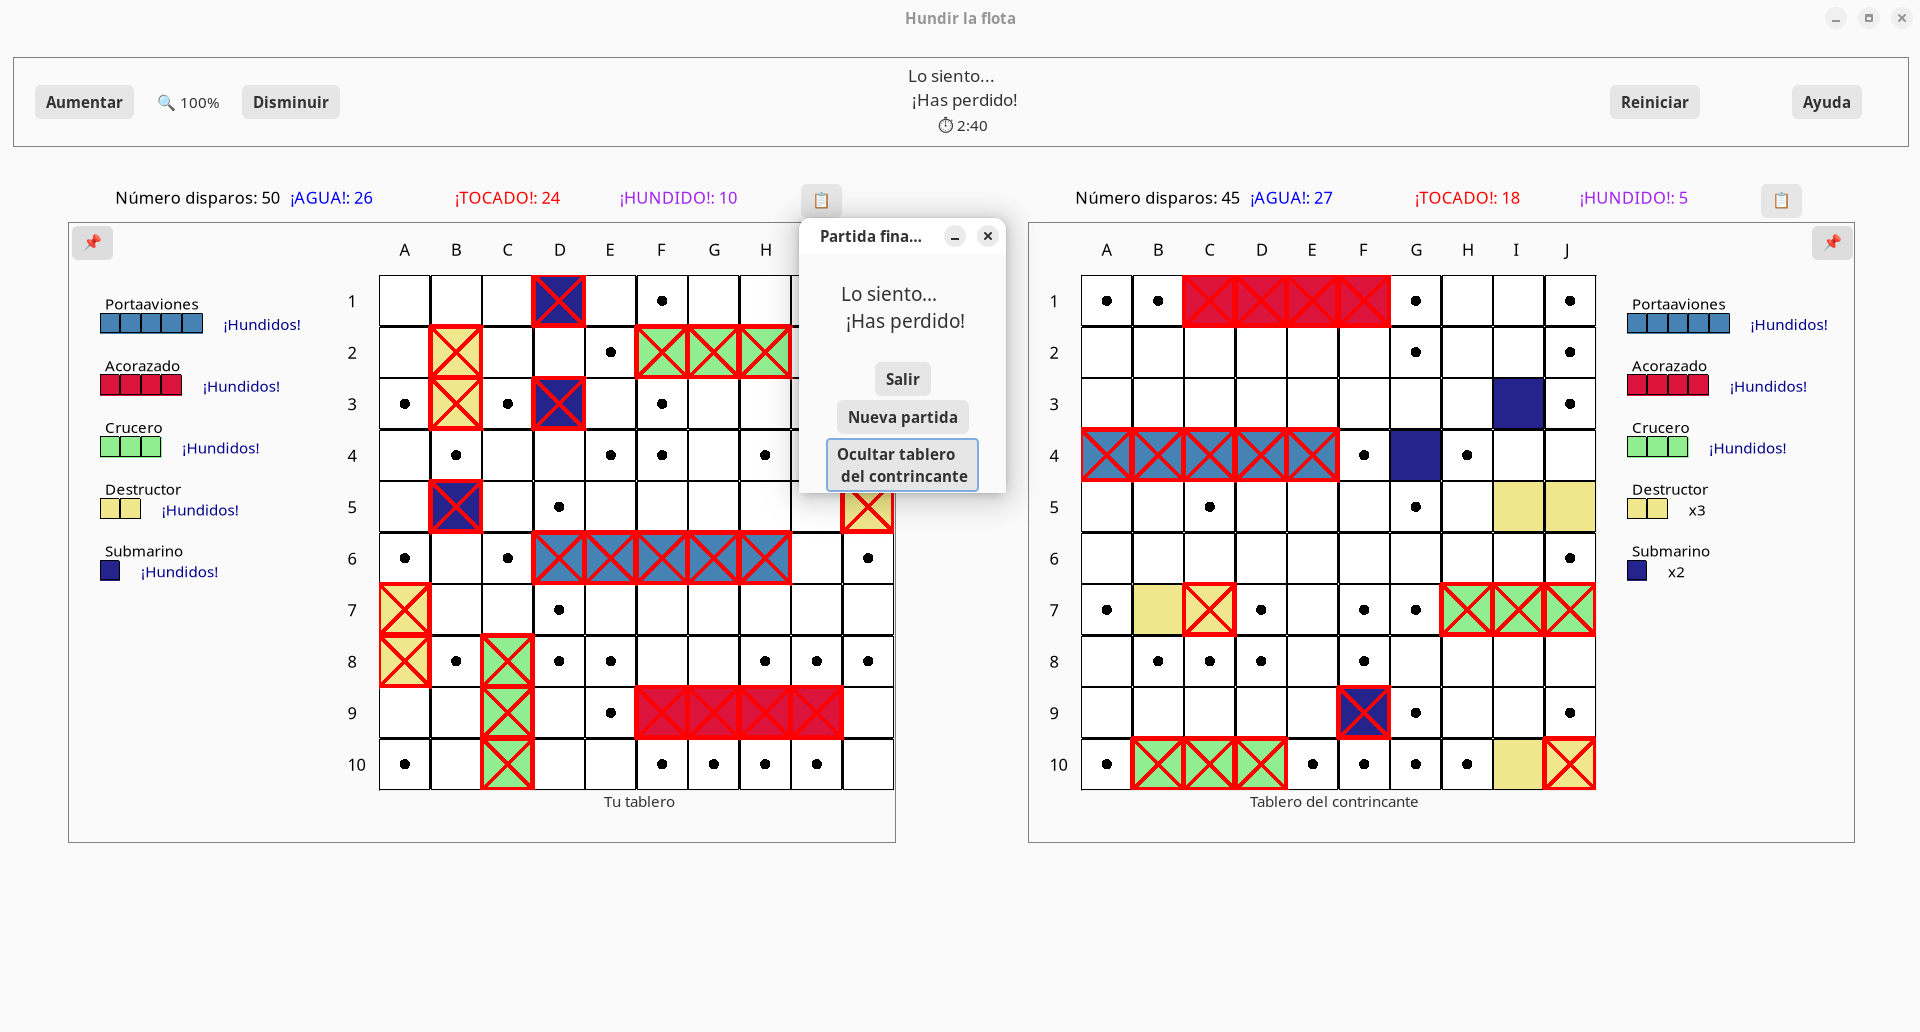
\includegraphics[width = \textwidth]{imagenes/resultados/mostrarTablero.png}}
            \caption{Mostrar el tablero de la CPU al finalizar}
          \end{figure}
      \end{columns}
\end{frame}



\section{Conclusiones}

\begin{frame}
    \frametitle{\insertsection}
    \framesubtitle{\hskip30pt \insertsubsection}

    \begin{block}{}
       Racket es un lenguaje diferente diseñado para ser usado con la programación declarativa,
       pero no ha quedado duda que es lo suficientemente potente e intuitivo como 
       cualquier otro lenguaje más popular.
    \end{block}
       
    \begin{block}{}
       Sus librerías gráficas, \emph{GUI} y \emph{Draw} permiten 
       construir aplicaciones de forma sencilla y deja la puerta abierta para indagar más profundamente
       si se necesita desarrollar características más complejas.
    \end{block}

    \begin{block}{}
       Usar Racket como lenguaje para desarrollar aplicaciones está a la altura de otros \textit{frameworks}
       como \textit{Qt} o \textit{Gtk}.
    \end{block}
    
\end{frame}


\section{Referencias}


\begin{frame}{Referencias}
\begin{block}{Sitios de interés:}
\begin{thebibliography}{10}

\bibitem[mot,4]{MOT}
\textcolor{black}{Racket Documentation (v8.11)}\\
\emph{\href{https://docs.racket-lang.org/gui/index.html}{The Racket Graphical Interface Toolkit}}\\
\textcolor{black}{Consultado el 11 de enero de 2024}

\bibitem[mot,6]{MOT}
\textcolor{black}{Racket Documentation (v8.11)}\\
\emph{\href{https://docs.racket-lang.org/draw/index.html}{The Racket Drawing Toolkit}}\\
\textcolor{black}{Consultado el 11 de enero de 2024}

\bibitem[mot,7]{MOT}
\emph{\href{https://en.wikipedia.org/wiki/Battleship_(game)}{Battleship}} \textcolor{black}{(s.f.)}\\
\textcolor{black}{Obtenido de enciclopedia libre Wikipedia}\\
\textcolor{black}{Consultado el 11 de enero de 2024}

\end{thebibliography}
\end{block}
\end{frame}



\begin{frame}{Referencias}
\begin{block}{Sitios de interés:}
\begin{thebibliography}{10}

\bibitem[mot,8]{MOT}
\textcolor{black}{James W. Stelly (2021)}\\
\emph{\href{https://www.google.es/books/edition/Racket_Programming_the_Fun_Way/u54LEAAAQBAJ?hl=es&gbpv=0}{Racket Programming the Fun Waye}}\\
\textcolor{black}{Consultado el 11 de enero de 2024}

\bibitem[mot,8]{MOT}
\textcolor{black}{Nick Berry (2011)}\\
\emph{\href{http://www.datagenetics.com/blog/december32011/}{Battleship algorithms}}\\
\textcolor{black}{Consultado el 11 de enero de 2024}

\bibitem[mot,8]{MOT}
\textcolor{black}{Aydin Schwartz (2022)}\\
\emph{\href{https://towardsdatascience.com/coding-an-intelligent-battleship-agent-bf0064a4b319}{Coding an Intelligent Battleship Agent}}\\
\textcolor{black}{Consultado el 11 de enero de 2024}

\end{thebibliography}
\end{block}
\end{frame}

\begin{frame}{Referencias}
\begin{block}{Sitios de interés:}
\begin{thebibliography}{10}

\bibitem[mot,8]{MOT}
\textcolor{black}{PLT (Version 200, June 2002)}\\
\emph{\href{https://www.uco.es/users/ma1fegan/Comunes/asignaturas/pd/PLT/Scheme-misclib.pdf}{PLT Miscellaneous Libraries: Reference Manua}}\\
\textcolor{black}{Consultado el 11 de enero de 2024}

\bibitem[mot,8]{MOT}
\textcolor{black}{Francisco Javier Rodríguez Lozano (Curso académico 2013 - 2014. UCO)}\\
\emph{Representación Gráfica en Scheme}\\
\textcolor{black}{Consultado el 11 de enero de 2024}

\end{thebibliography}
\end{block}
\end{frame}


\begin{frame}{Referencias}
\begin{block}{Sitios de interés:}
\begin{thebibliography}{10}

\bibitem[mot,8]{MOT}
\textcolor{black}{battleship-game.org}\\
\emph{\href{https://battleship-game.org/}{Hundir la flota online}}\\
\textcolor{black}{Consultado el 11 de enero de 2024}

\bibitem[mot,8]{MOT}
\textcolor{black}{Domingo Gallardo}\\
\emph{\href{https://domingogallardo.github.io/apuntes-lpp/seminarios/seminario1-scheme/seminario1-scheme.html}{Seminario de Scheme}}\\
\textcolor{black}{Consultado el 11 de enero de 2024}


\bibitem[mot,8]{MOT}
\textcolor{black}{Philip F.}\\
\emph{\href{https://boardgames.stackexchange.com/questions/56427/strategies-in-battleship}{Strategies in battleship}}\\
\textcolor{black}{Consultado el 11 de enero de 2024}



\end{thebibliography}
\end{block}
\end{frame}

\begin{frame}{Referencias}
\begin{block}{Sitios de interés:}
\begin{thebibliography}{10}

\bibitem[mot,8]{MOT}
\textcolor{black}{Bas Steunebrink}\\
\emph{\href{https://groups.google.com/g/racket-users/c/uAfGFOTh3J8}{Create executable for "Pretty Big" legacy program}}\\
\textcolor{black}{Consultado el 11 de enero de 2024}

\bibitem[mot,8]{MOT}
\textcolor{black}{u/fazzah}\\
\emph{\href{https://www.reddit.com/r/dataisbeautiful/comments/4m0vut/battleship_game_algorithm_comparison_with_results/}{Battleship game algorithm comparison with results}}\\
\textcolor{black}{Consultado el 11 de enero de 2024}

\bibitem[mot,8]{MOT}
\textcolor{black}{Hasbro}\\
\emph{\href{https://www.hasbro.com/common/instruct/battleship.pdf}{Battleship rules}}\\
\textcolor{black}{Consultado el 11 de enero de 2024}




\end{thebibliography}
\end{block}
\end{frame}





% \newpage

% \vspace*{2.9cm}
% \begin{block}{}
% \begin{center}
% \fontsize{20pt}{20pt} \selectfont {Gracias por su atención}
% \end{center}
% \end{block}


\end{document}
